\chapter{the Crossing tree and $H$-sssi processes} % (fold)
\label{cha:the_crossing_tree_and_h_sssi_processes}

Inspired by the simplicity of the statistical properties of the crossing tree for
Brownian motions we formulate the following conjecture: whenever $\{X(t)\}$ is a
continuous $H$-sssi process, then $X(0)= 0$ almost surely and the process is uniquely
identified by the statistical properties of the crossing tree, namely the crossing
durations, the excursion and the offspring distributions in the following way:\\
\noindent \textbf{Conjecture}\begin{itemize}
    \item The random variables $Z_k^n$ are possibly correlated, but nevertheless
    identically distributed, with probability distribution
    \[ \pr\bigl(Z_k^n=2m\bigr) = 2^{1-H^{-1}}\bigl(1-2^{1-H^{-1}}\bigr)^{m-1} \,,\]
    for all $m\geq 1$;
    \item The distribution of excursion directions $V_k^n$ (orientation patterns),
    conditional on the orientation of the parent crossing, is:
    \[ \pr\bigl( +- \bigr.\bigl\lvert ++ \bigr)
	= \pr\bigl( -+ \bigr.\bigl\lvert -- \bigr)
	= 2^{-2H^{-1}} \,.; \]
	\item The properly scaled crossing durations $4^{-\sfrac{n}{2H}} W_k^n$
	are identically distributed with finite variance;
\end{itemize}
% The rationale behind the scaling in the crossing duration case is given below. By
% definition, the duration of a crossing of grid $\delta 2^n \mathbb{Z}$ (level-
% $n$ crossing duration, denoted here by $\tau_n$) is the time needed for the process
% $\{X(t)\}$ to move from some value $X(t)$ to $X(t+\tau_n) = 2^n X(t)$. Therefore one
% can use self-similarity for the following chain of thought:
% \[ X(\tau_n) \overset{\Dcal}{\sim} 2^n X(\tau_1) \overset{\Dcal}{\sim} 2^n \tau_1^H X(\tau_1) \,, \]
% whence follows that $\tau_n^H X(1) \overset{\Dcal}{\sim} 2^n \tau_1^H X(\tau_1)$. This
% observation gives an idea of how should the crossing durations between different
% tree level be related.

In order to gather empirical evidence either supporting or refuting this claim,
extensive numerical study was in order. The Monte-Carlo simulation was performed
on each of the processes mentioned in the previous chapter (p.~\pageref{cha:h_sssi_processes}).
The software part of the experiment was implemented in Python in conjunction with
Numpy and FFTW, a standalone open source library dedicated to efficiently computing
Fast Fourier Transforms using .\footnote{The source code of the developed toolkit for crossing tree
construction and analysis is publicly available online at
\url{https://github.com/ivannz/study_notes/tree/master/year_14_15/course_project/release}}

% chapter the_crossing_tree_and_h_sssi_processes (end)

\section{Generation of fBm, Hermite and Weierstrass processes} % (fold)
\label{sec:generation_of_fbm_hermite_and_weierstrass_processes}

The basic building block of the fBm and the Hermite processes is a Gaussian noise with a
particular correlation structure, as evidenced by the stochastic integral representations
of these processes. All processes generated for this study were discrete versions of
the corresponding continuous processes.

Generation of the fractional Brownian motion for this study is based on the Circulant
Embedding method of Dietrich and Newsam for generating fractional Gaussian noise (fGn),
\cite{WRCR:WRCR6232}. In short, the method utilizes the structure of the correlation
matrix of fGn to embed it into a larger circulant Toeplitz matrix, suitable for
imposing the required covariance structure upon independent standard normal random
variables via standard forward Discrete Fourier Transform. For details the reader
is encouraged to refer to the original paper~\cite{WRCR:WRCR6232} and a more recent
one~\cite{Perrin:1058211}.

As for the Hermite processes, synthesis of their sample path was based on the fundamental
theorem of Lamperti (see~\cite{embrechtsselfsimilar}) which states that $H$-sssi
processes are the only limiting law of normalized partial sum of a stationary random
sequence. Formally, if $(X_i)_{i\geq1}$ is stationary and for some regularly varying
function $a_n\to \infty$ and the following limiting exists
\[ \frac{1}{a_n} \sum_{i=1}^{[nt]} X_i \overset{\Dcal}{\rightarrow} y(t) \,, \]
where convergence is in finite-dimensional distributions, then the limiting process
$(Y_t)_{t\geq0}$ is $H$-sssi for some $H>0$.

For instance, if $(X_i)_{i\geq 1}$ is an independent and identically distributed,
sequence, then the limit of normed partial sums is the Brownian motion, which is
$\frac{1}{2}$-sssi. In case if the stationary sequence $X_i$ is \textbf{l}ong-
\textbf{r}ange \textbf{d}ependent, i.e. with slowly decaying autocorrelation,
the limit $Y(t)$ is often some $H$-sssi process with $H>\frac{1}{2}$ (see~\cite{embrechtsselfsimilar}).
In particular if $X_i = \xi_i^2 -1$ for some stationary Gaussian sequence with
$\xi_i\sim\mathcal{N}(0,1)$, but $\ex(\xi_1\xi_{n+1}) = n^{H-1}L(n)$ as $n\to \infty$
for some $H\in(\tfrac{1}{2},1)$ and some slowly varying function $L$, then the
limiting process is a non-Gaussian $H$-ss process with strongly dependent, yet
stationary increments corresponding to a Hermite process of order $2$ (see~\cite{embrechts2000introduction}).
The transformation used to compute $(X_i)_{i\geq0}$ form $(\xi_i)_{i\geq0}$ is
the $2$-nd order Hermite polynomial.

Sample paths of the Weierstrass process were simulated on a uniformly spaced grid
$(t_k)_{i=0}^N\in [0,1]$ with $0 = t_0< t_1 < \ldots < t_{N-1} < t_N = 1$. The spacing
of the grid and the fundamental harmonic $\lambda_0$ were chosen so that the trigonometric
functions are adequately sampled over the unit interval (see ~\cite{decrouez2013estimation}).

% section generation_of_fbm_hermite_and_weierstrass_processes (end)

\section{Simulation results} % (fold)
\label{sec:results}

In order to study the empirical support of the hypothesised statistical properties of
the crossing tree as well as see how accurate in practice the crossing tree methodology
confirms the theoretical result in \cite{ECP1673}, an extensive Monte-Carlo experiment
was preformed.

The crossing trees were constructed for a base scale $\delta$ dependent on each particular
sample realisation of the process, but in such a way as to enable meaningful comparisons
of the crossing tree properties between different Monte-Carlo replications and between
different classes of $H$-sssi processes. For a particular sample path $(x_j)_{j=0}^N$
of the process $\{X(t)\}$ the base scale was set to
\[ \delta = \text{med}\bigl( |\Delta x_j| \bigr) \,, \]
where $\Delta x_j = x_j - x_{j-1}$ and $\text{med}(\cdot)$ is the median of the
sample. The rationale behind the median of absolute increments of the sample path
was to strike a balance between the biasedness of the crossing tree parameters,
resulting from linear interpolation of the crossing times and the inaccuracy due to
too coarse a resolution. Other choices for the base scale were considered, such
as the standard deviation and the \textbf{i}nter\textbf{q}uartile \textbf{r}ange
measure of statistical dispersion of the increments. Neither did produce any significantly
different results from the median, except only that they tended to produce trees with
fewer levels and thus cover a narrower range of resolutions of the process.

It seems natural to begin with the study of the fractional Brownian motion. To this end,
$10^3$ Monte-Carlo simulations of sample paths of the fBm process were simulated. The
process was confined to the unit interval and discretized to have $2^{21}$ sample points.

Before proceeding to the evaluation of statistical properties of the crossing trees,
it is necessary to determine the range of tree levels (grid scales, or resolutions)
for which self-similarity is apparent.
\begin{figure}[htb]\begin{center}
    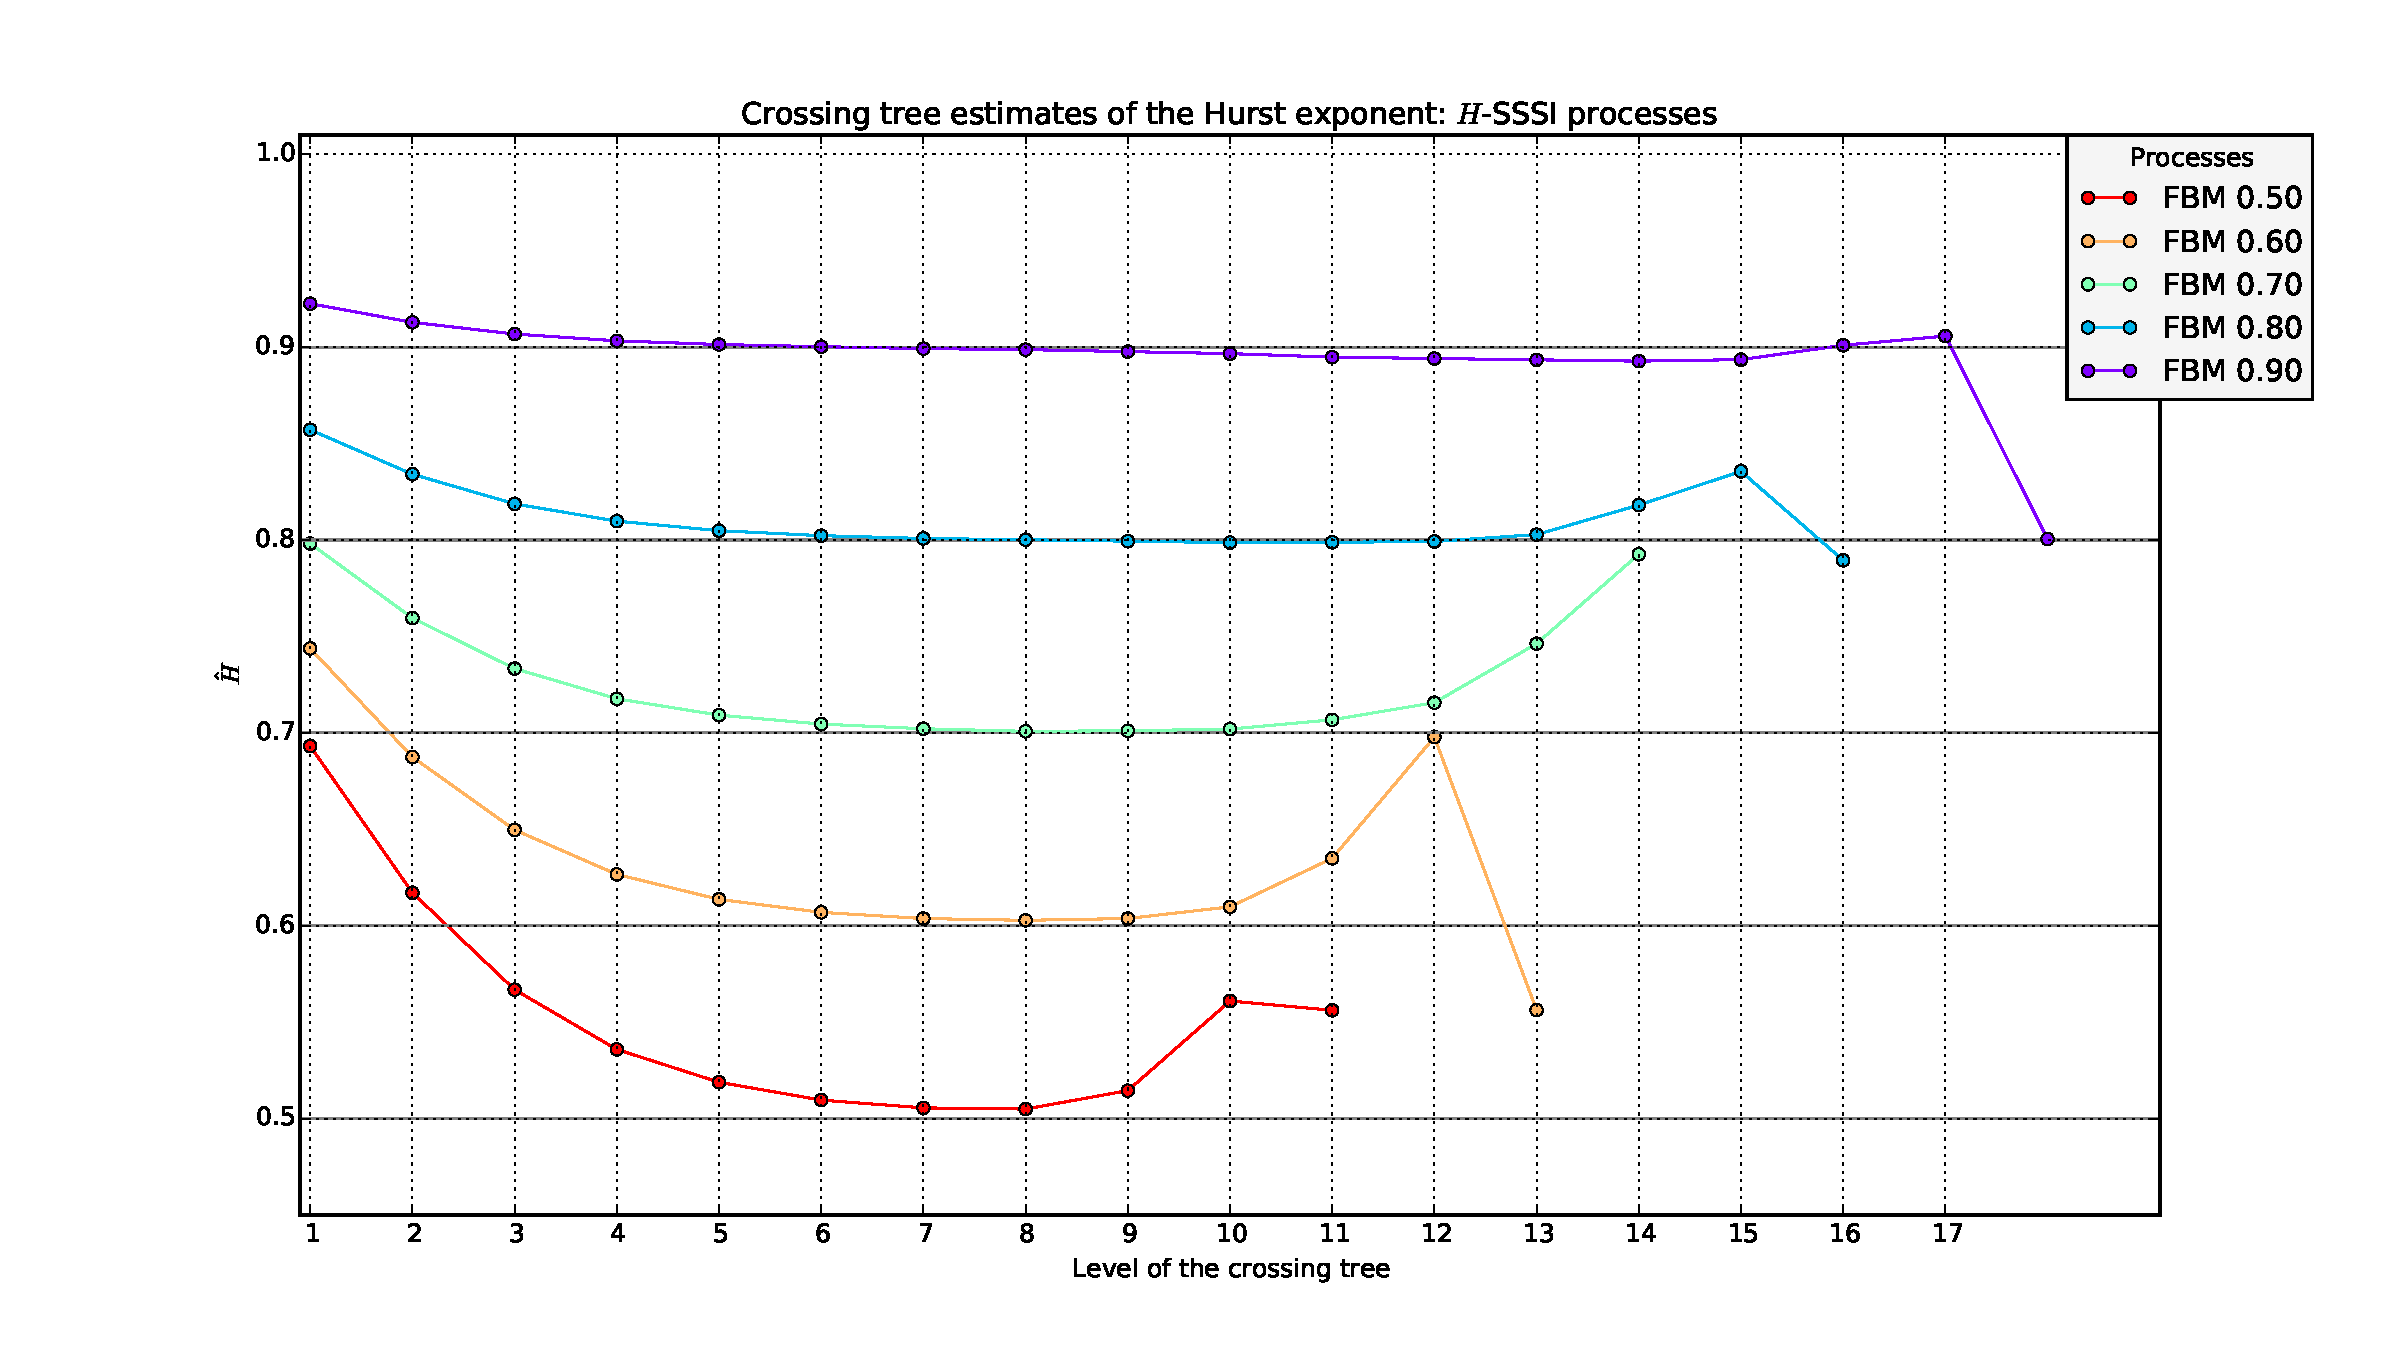
\includegraphics[width=6in]{images/fbm_fig_05_med_1000-21}
    \caption{The plot of the estimates of the Hurst index $H$ on the offspring data
    of a single level of the crossing tree based on $10^3$ Monte-Carlo simulations of
    fBm.}
\label{fig:fbm_hurst_crossing_tree}
\end{center}\end{figure}

Figure~\ref{fig:fbm_hurst_crossing_tree} suggests that scale-invariance properties
for the studied fractional processes and the chosen method of computation of the
base scale manifest their effects at across levels from 6 to 9. In fact the $\chi^2$
test described in section~\ref{sec:analysis_using_the_crossing_tree} does not seem
to support this finding and instead has the lowest empirical rejection rate exactly
at levels from 7 to 8 (see table~\ref{tbl:chi_sq_test_for_fbm_only}).
\begin{table}[h]\begin{center}
	\begin{tabular}{l||c|c|c|c|c|c|}
	Process 		&  $6-7$ &          $7-8$ & $8-9$ &  $6-8$ &  $7-9$ &  $6-9$ \\ \hline\hline
	fBm-$0.50$ 		& $10.6$ & $\mathbf{8.2}$ & $9.1$ & $13.6$ & $12.2$ & $16.2$ \\ \hline 
	fBm-$0.60$ 		& $10.9$ & $\mathbf{9.1}$ & $9.4$ & $14.2$ & $13.1$ & $16.4$ \\ \hline 
	fBm-$0.70$ 		&  $9.4$ & $\mathbf{7.0}$ & $7.2$ & $12.6$ & $11.2$ & $15.8$ \\ \hline 
	fBm-$0.80$ 		& $10.3$ & $\mathbf{6.1}$ & $6.7$ & $12.8$ & $10.7$ & $16.9$ \\ \hline 
	fBm-$0.90$ 		& $11.1$ & $\mathbf{7.8}$ & $7.9$ & $18.0$ & $12.8$ & $27.7$ \\ \hline 
 	\end{tabular}
	\caption{The table of empirical rejection rate at significance level of $\alpha = 5\%$
	of the $\chi^2$ test for self-similarity between levels of the crossing tree. }
\label{tbl:chi_sq_test_for_fbm_only}
\end{center}\end{table}
Since the self-similarity of the simulated fractional Brownian motion paths seems
to become apparent at levels 7 and 8 on average, we pool the crossing tree data of
these levels in order to obtain more reliable estimates.

Restricting the attention to the Brownian motion case (fBm with $H=\tfrac{1}{2}$)
one can easily see that the numerical evidence is well aligned with the theoretical
result of Jones and Rolls (fig.~\ref{fig:fbm_offspring_distribution}).
\begin{figure}[htb]\begin{center}
    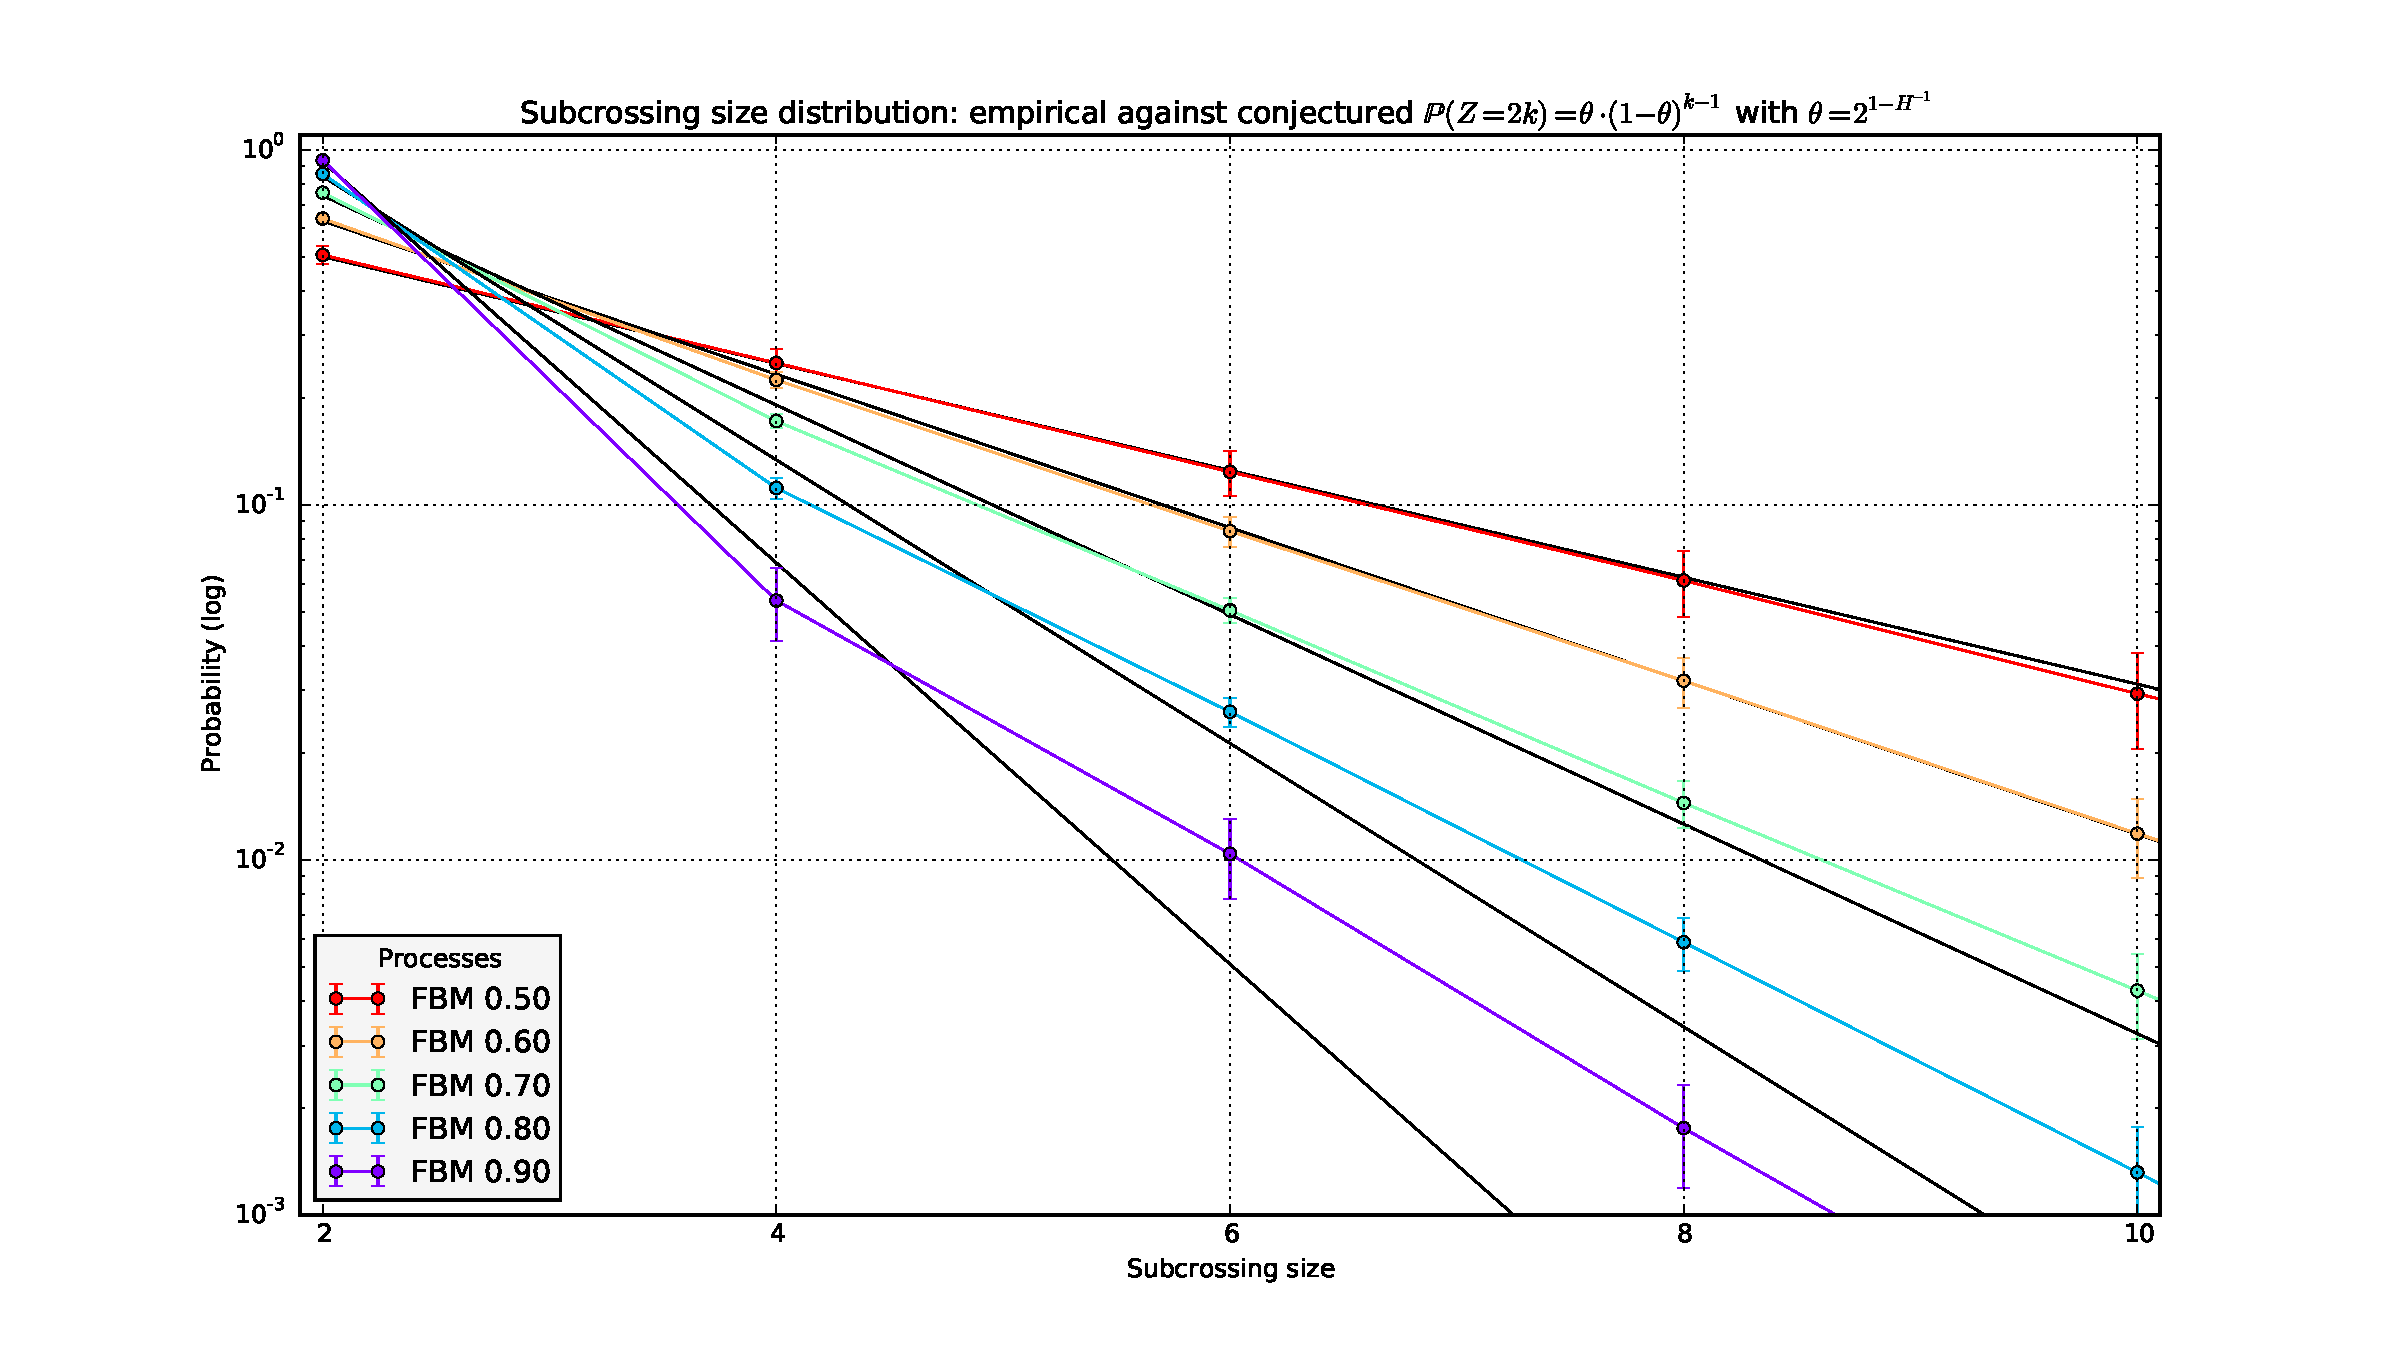
\includegraphics[width=6in]{images/fbm_fig_01_med_1000-21}
    \caption{The log-plot of the offspring distributions estimated on 1000 sample discrete paths
    of the fBm process of length $2^{21}$ and Hurst exponents in the range from $0.5$ to $0.9$.}
\label{fig:fbm_offspring_distribution}
\end{center}\end{figure}
Similarly, the theoretical probability of an up-down crossing conditional on an upcrossing
is matched very closely by the numerical evidence (fig.~\ref{fig:fbm_offspring_up_down}).
The results are similar in the down-up excursions case (fig.~\ref{fig:fbm_offspring_down_up}).

\begin{figure}[htb]\begin{center}
    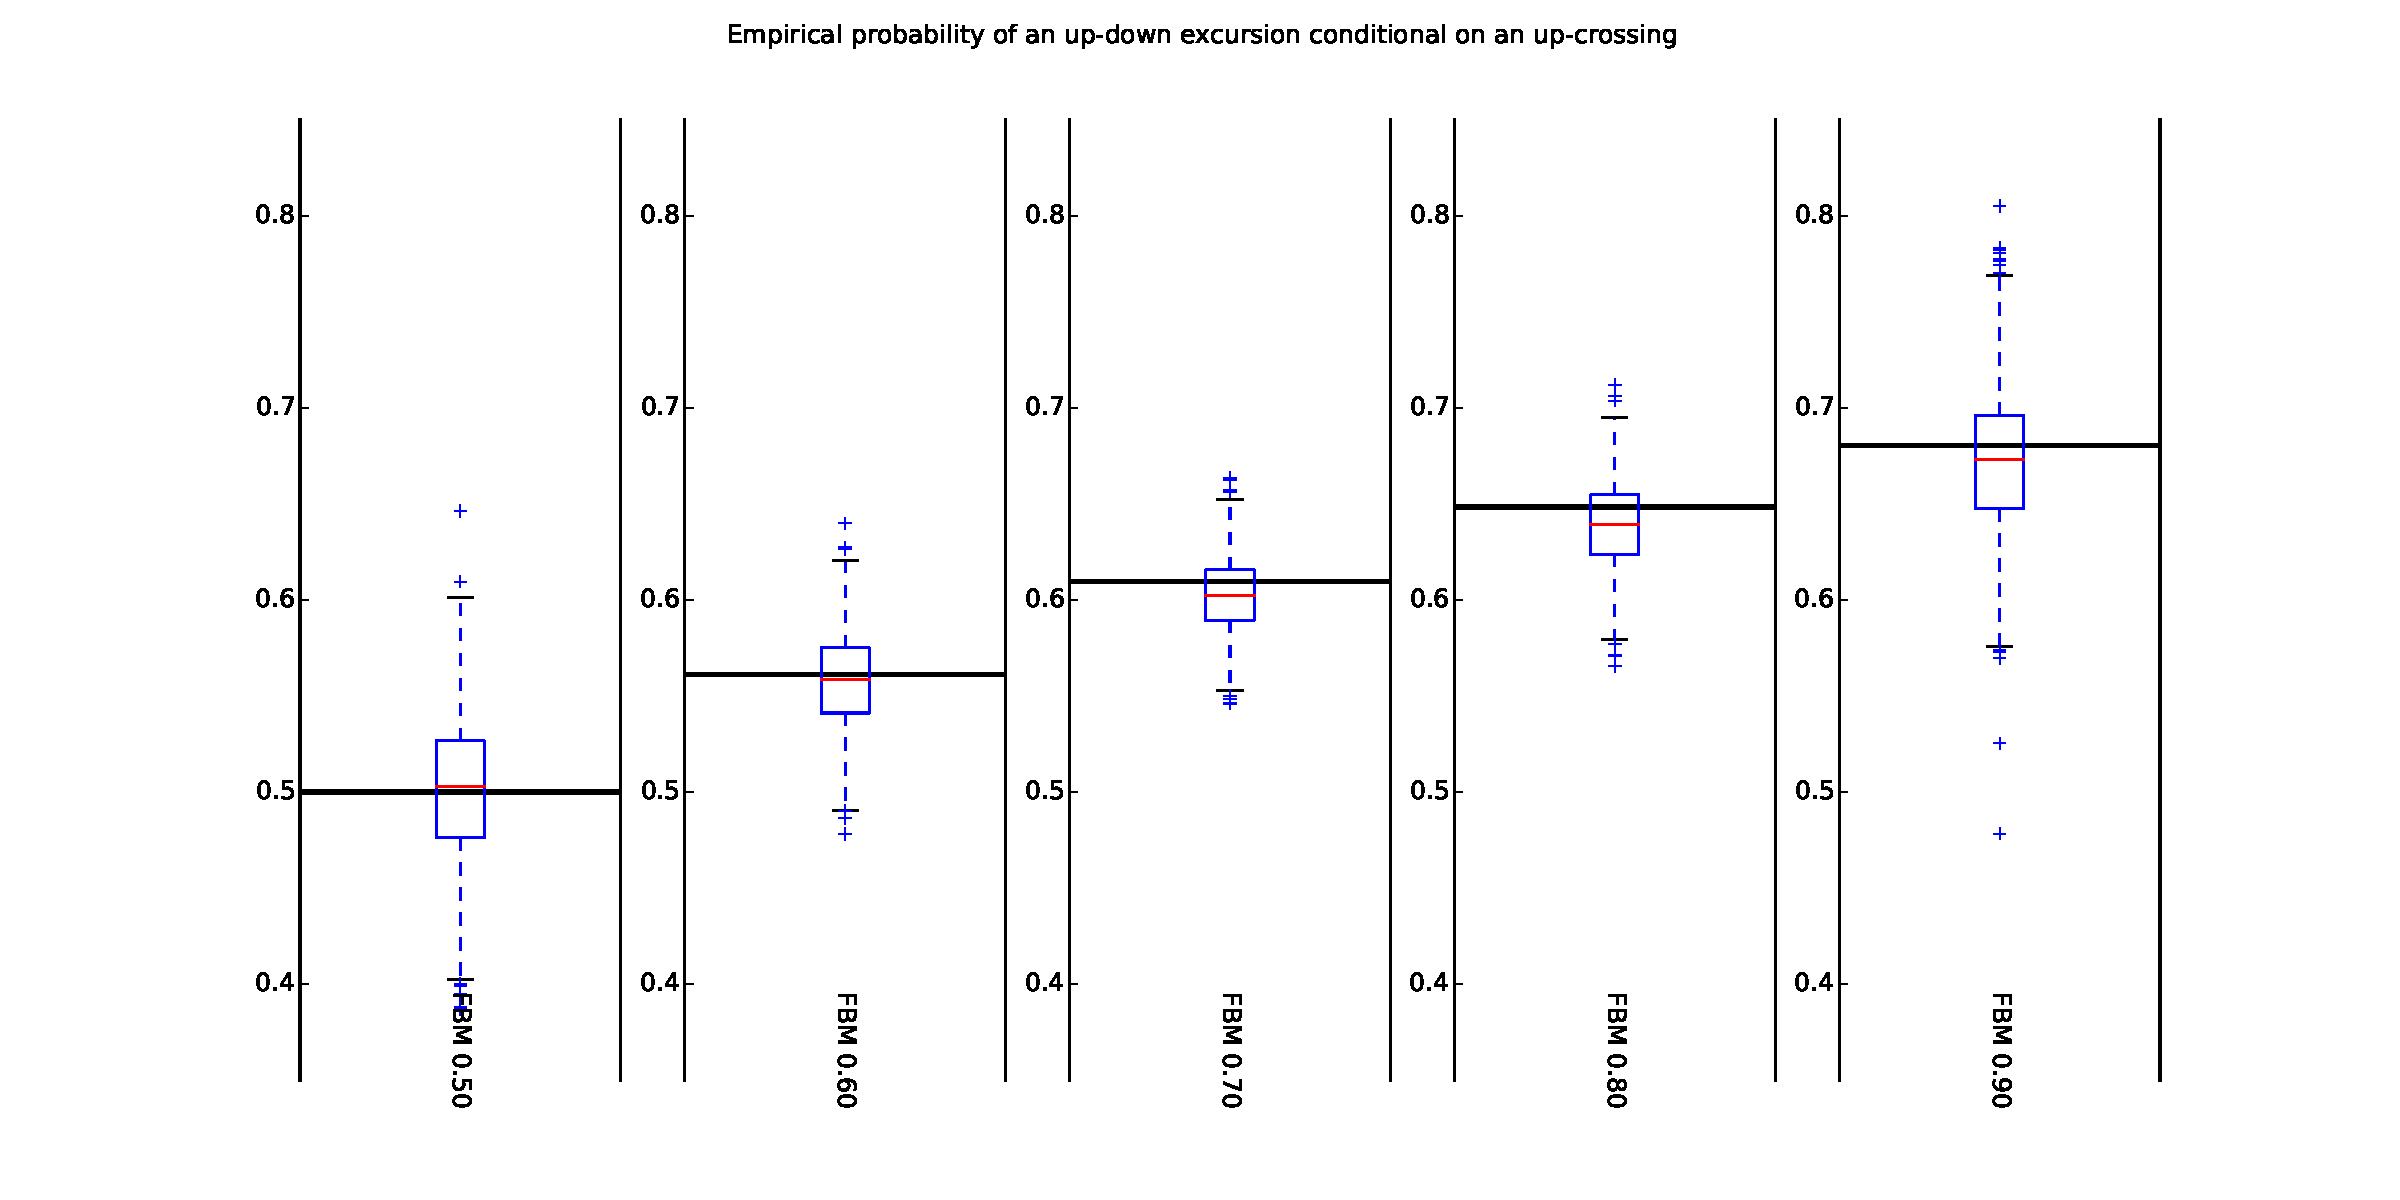
\includegraphics[width=6in]{images/fbm_fig_03_up-down_med_1000-21}
    \caption{The estimated conditional probability of an up-down excursion given upward
    orientation of the parent crossing.}
\label{fig:fbm_offspring_up_down}
\end{center}\end{figure}

\begin{figure}[htb]\begin{center}
    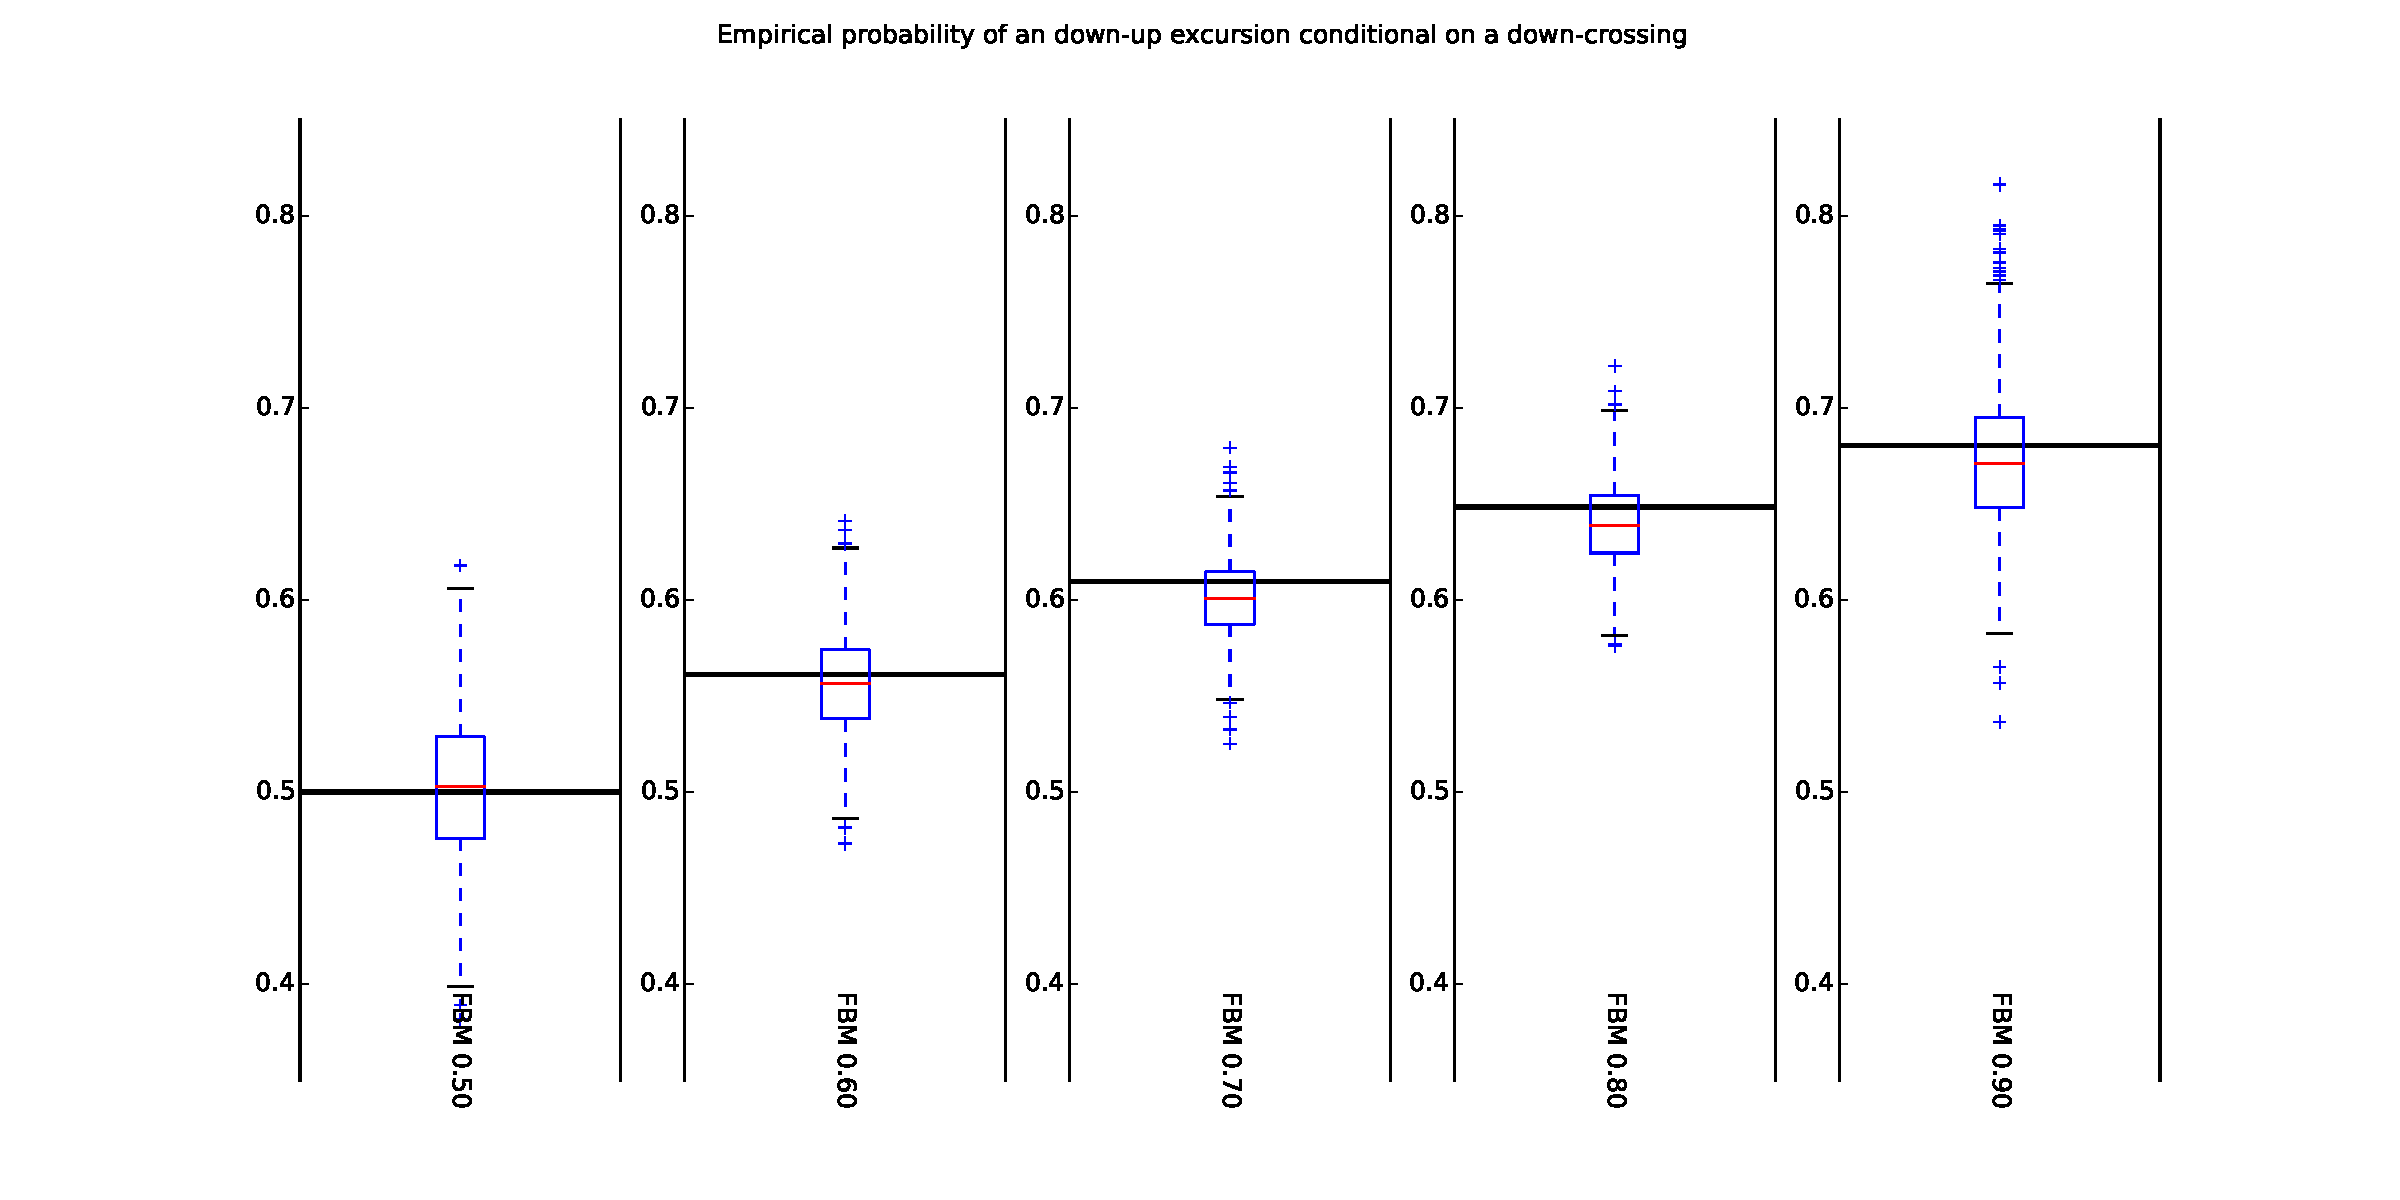
\includegraphics[width=6in]{images/fbm_fig_03_down-up_med_1000-21}
    \caption{The box-plot of the estimates of the probability of an down-up excursion
    conditional on the orientation of the parent crossing being downward.}
\label{fig:fbm_offspring_down_up}
\end{center}\end{figure}

As for the conjectured distribution, the offspring distribution in the performed
experiments seems to suggest that the levels of the tree, at least for the fractional
Brownian motion, tend to be populated by crossings with more than predicted number
of subcrossings (see tables~\ref{tbl:empirical_probs_01} for $H=0.6$
and~\ref{tbl:empirical_probs_02} for $H=0.8$). However the failure of the conjectured
crossing size distribution to match the empirical results closely, should not be
considered as a serious evidence against it in this case. Indeed, the empirical
offspring distribution for fBm with $H=0.5,0.6$ and $0.7$ is aligned quite well
with the conjecture, and since there is no theoretical reason as to why the
dependence on $H$ should break down for values of $H$ closer to $1$, we attribute
this discrepancy to numerical issues of discretizing continuous processes and
simulating fGn with long range dependence. 

Finally, the mean crossing durations, averaged for each replication across all detected
crossings of a single level indeed demonstrate plausibility of the conjectured scaling
between levels of the crossing tree, see fig.~\ref{fig:fbm_avg_crossing_durations} for fBm.
\begin{figure}[htb]\begin{center}
    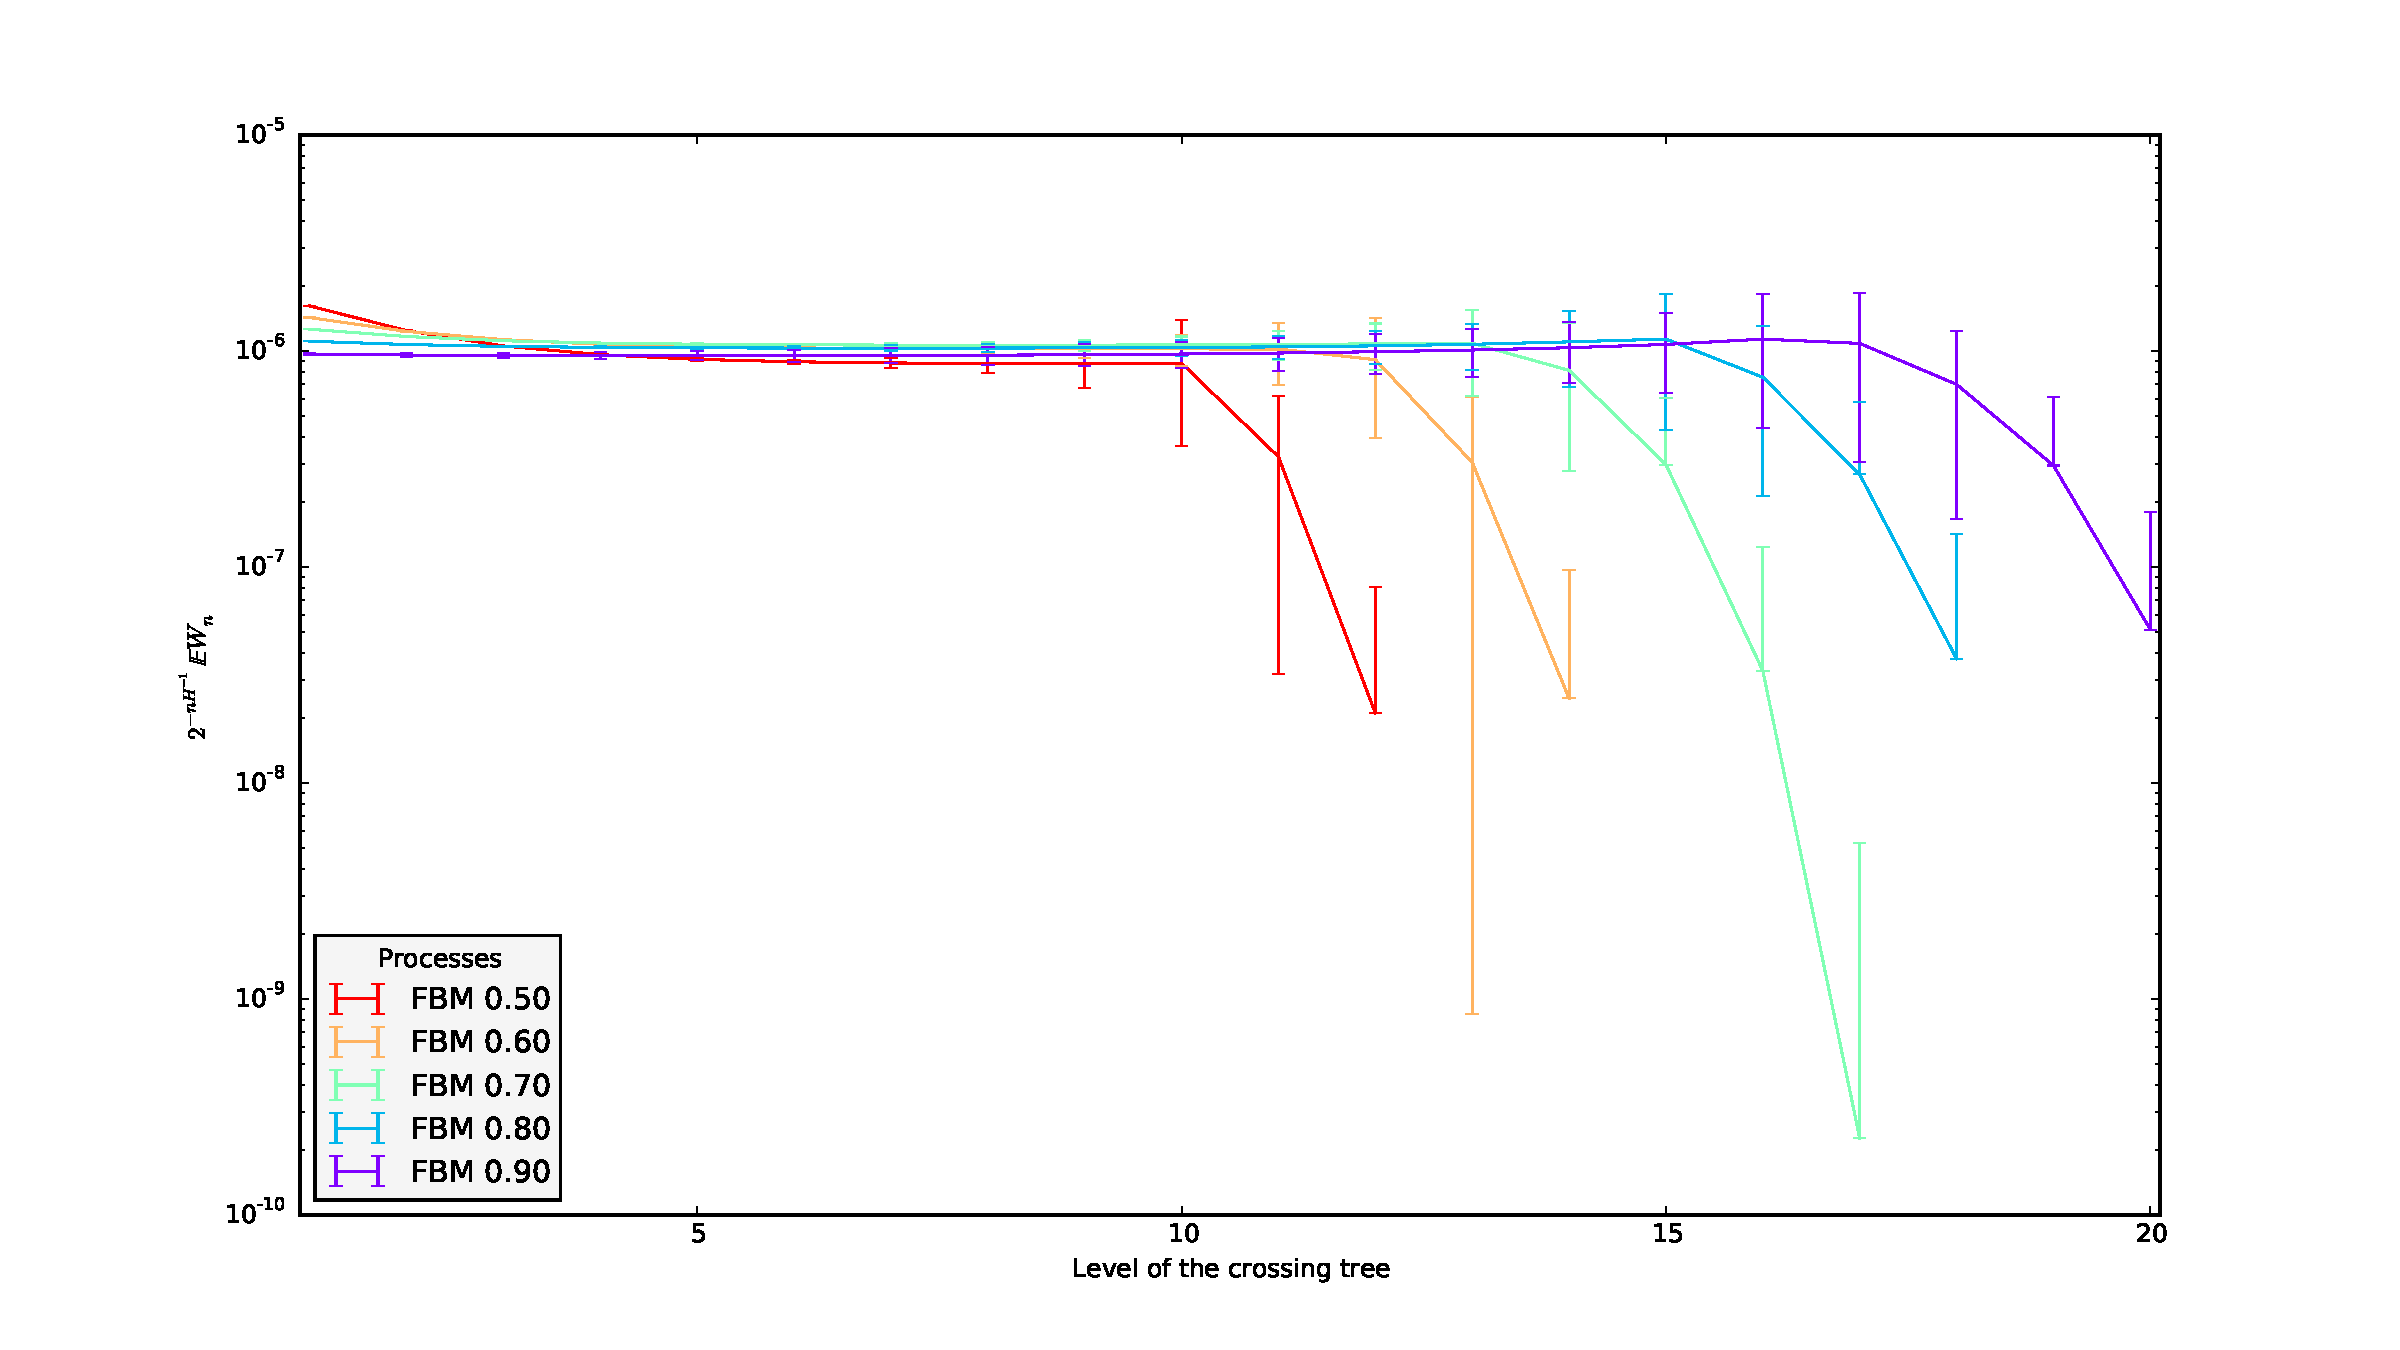
\includegraphics[width=6in]{images/fbm_fig_08_med_1000-21}
    \caption{The average crossing duration at each level of the crossing tree built
    for fractional Brownian motion processes.}
\label{fig:fbm_avg_crossing_durations}
\end{center}\end{figure}

Now let's turn to the Hermite and Weierstrass processes. This time $10^4$ random
replications of sample paths of size $2^{17}$ were generated for each process.
This size limitation was dictated by deteriorating numerical accuracy of the procedure,
responsible for generating sample paths of Hermite processes. Thus in order to produce
comparable results, sample paths of fBm and Weierstrass processes were limited to $2^{17}$
points as well.

Figure~\ref{fig:all_hurst_crossing_tree} suggests that the processes studied share common
statistical properties of the crossing tree.
\begin{figure}[htb]\begin{center}
    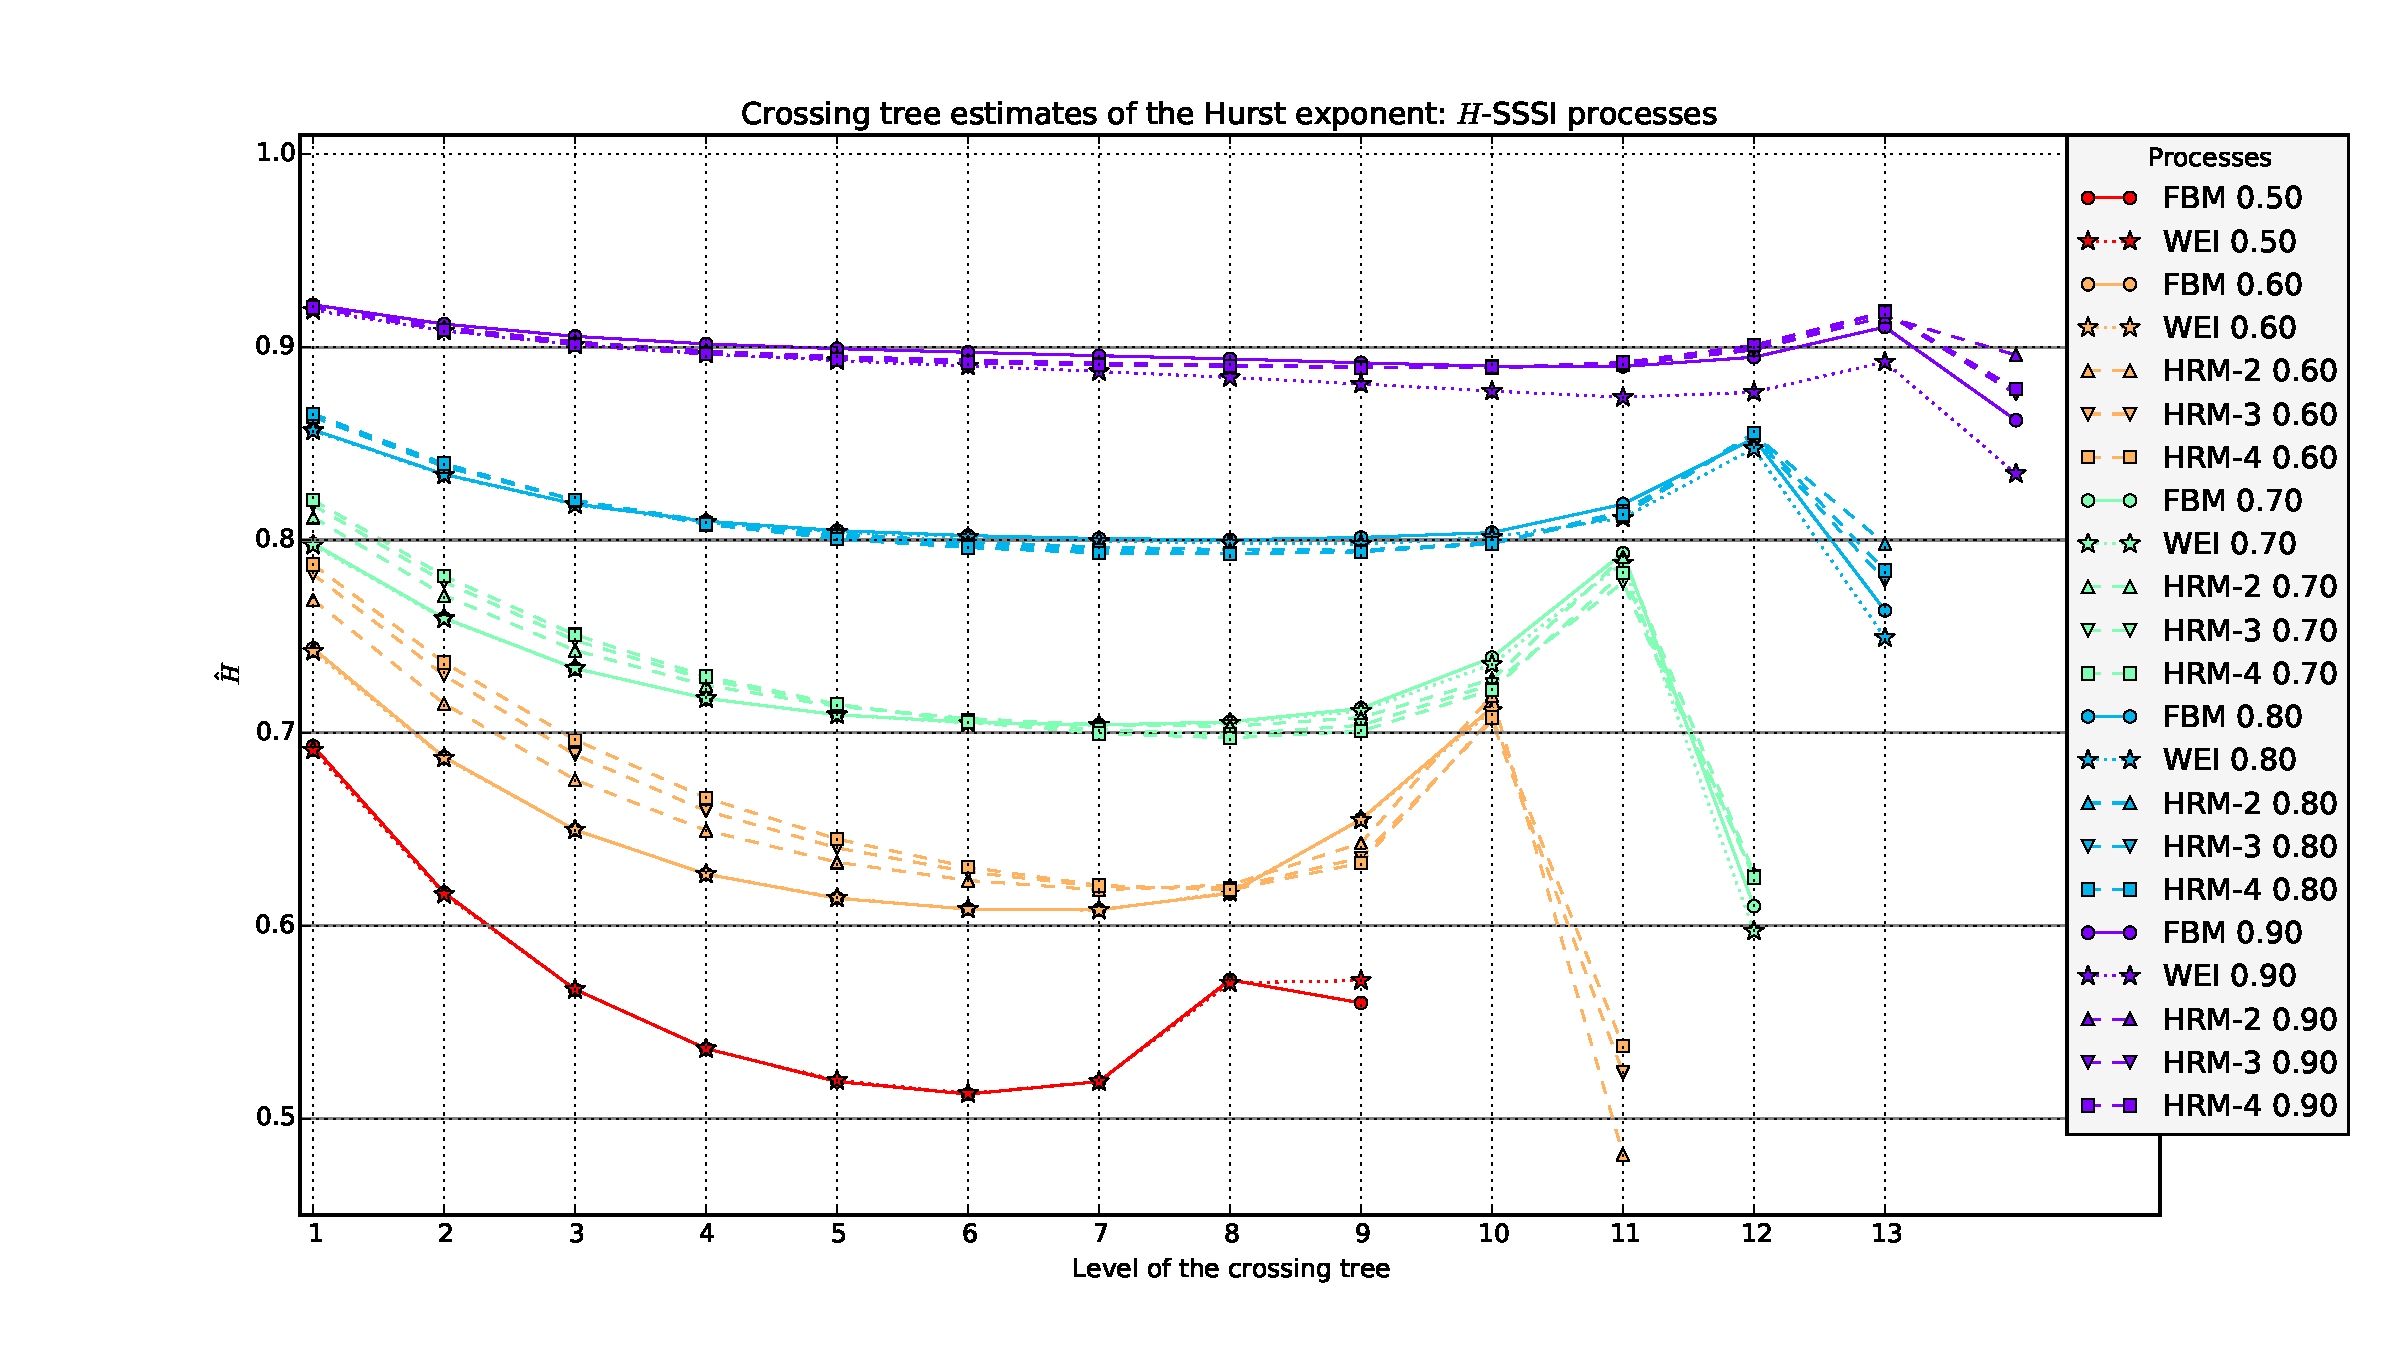
\includegraphics[width=6in]{images/fig_05_med_10000-17}
    \caption{Estimates of the Hurst exponent $H$ based on a single level of the crossing tree for
    the all studied $H$-sssi processes.}
\label{fig:all_hurst_crossing_tree}
\end{center}\end{figure}

Table~\ref{tbl:chi_sq_test_for_all_01} summarizes the empirical rejection rates of
the $\chi^2$ test for self similarity across the range of levels indicated in the
header of the table.
\begin{table}[h]\begin{center}
	\begin{tabular}{l||c|c|c|c|c|c|}
	Process 		& $6-7$ &  $7-8$ &  $8-9$ &  $6-8$ &  $7-9$ &  $6-9$ \\ \hline\hline
	  fBm-$0.50$	& $9.7$ & $15.7$ &     -- & $13.8$ &  $\mathbf{3.6}$ &  $5.4$ \\ \hline
	  fBm-$0.60$	& $8.8$ &  $9.3$ &  $\mathbf{5.6}$ & $14.2$ & $14.3$ & $16.5$ \\ \hline
	  fBm-$0.70$	& $7.6$ &  $\mathbf{6.6}$ & $10.5$ & $13.4$ & $15.7$ & $17.8$ \\ \hline
	  fBm-$0.80$	& $6.5$ &  $4.8$ &  $\mathbf{4.5}$ & $11.5$ & $13.1$ & $16.5$ \\ \hline
	  fBm-$0.90$	& $\mathbf{4.5}$ &  $5.1$ &  $6.9$ & $11.7$ & $13.6$ & $19.8$ \\ \hline\hline

	  WEI-$0.50$	& $9.6$ & $12.4$ &     -- & $13.9$ &  $\mathbf{2.2}$ &  $5.1$ \\ \hline
	  WEI-$0.60$	& $\mathbf{8.2}$ &  $9.6$ & $11.1$ & $13.2$ & $14.8$ & $15.5$ \\ \hline
	  WEI-$0.70$	& $7.0$ &  $\mathbf{5.9}$ &  $\mathbf{5.9}$ & $12.9$ & $14.6$ & $15.8$ \\ \hline
	  WEI-$0.80$	& $6.2$ &  $5.5$ &  $\mathbf{4.9}$ & $13.1$ & $13.2$ & $17.0$ \\ \hline
	  WEI-$0.90$	& $5.0$ &  $\mathbf{1.9}$ &  $8.7$ & $12.2$ &  $9.7$ & $21.0$ \\ \hline\hline

	HRM-2-$0.60$ 	& $9.6$ &  $9.2$ &  $\mathbf{7.1}$ & $15.2$ & $15.9$ & $19.6$ \\ \hline
	HRM-2-$0.70$ 	& $8.5$ &  $\mathbf{7.4}$ & $11.3$ & $13.9$ & $15.1$ & $18.2$ \\ \hline
	HRM-2-$0.80$ 	& $6.5$ &  $\mathbf{5.4}$ &  $5.6$ & $12.5$ & $12.3$ & $17.8$ \\ \hline
	HRM-2-$0.90$ 	& $6.4$ &  $\mathbf{4.9}$ &  $0.0$ & $12.7$ & $14.5$ & $18.7$ \\ \hline\hline

	HRM-3-$0.60$ 	& $9.6$ &  $\mathbf{9.2}$ & $13.7$ & $15.6$ & $17.9$ & $20.3$ \\ \hline
	HRM-3-$0.70$ 	& $\mathbf{7.9}$ &  $8.1$ &  $\mathbf{7.9}$ & $14.5$ & $16.4$ & $19.2$ \\ \hline
	HRM-3-$0.80$ 	& $5.5$ &  $\mathbf{4.3}$ &  $5.4$ & $11.8$ & $13.1$ & $16.7$ \\ \hline
	HRM-3-$0.90$ 	& $\mathbf{5.6}$ &  $7.7$ & $12.5$ & $13.4$ & $14.1$ & $19.8$ \\ \hline\hline

	HRM-4-$0.60$ 	& $9.7$ &  $\mathbf{9.3}$ & $12.3$ & $16.5$ & $17.4$ & $21.4$ \\ \hline
	HRM-4-$0.70$ 	& $8.1$ &  $7.2$ &  $\mathbf{6.0}$ & $15.4$ & $16.8$ & $20.4$ \\ \hline
	HRM-4-$0.80$ 	& $5.7$ &  $7.4$ &  $\mathbf{1.8}$ & $11.7$ & $13.7$ & $16.8$ \\ \hline
	HRM-4-$0.90$ 	& $5.1$ &  $\mathbf{2.9}$ &  $8.3$ &  $9.8$ & $12.9$ & $19.0$ \\ \hline\hline

 	\end{tabular}
	\caption{The table of empirical rejection rate at significance level of $\alpha = 5\%$
	of the $\chi^2$ test for self-similarity between levels of the crossing tree. }
\label{tbl:chi_sq_test_for_all_01}
\end{center}\end{table}
There does not seem to be a common range of levels, at the corresponding resolutions of which
all processes exhibit scale-invariance. This might be attributed to the fact that the path
of the generated processes were insufficiently long to adequately populate the higher
levels of the crossing tree. Nevertheless, it seems reasonable to expect a certain degree
of self-similarity over levels from 7 to 8, which with due caution, could yield empirical
evidence useful for analysing the conjecture.

Indeed, the offspring distribution plot (fig.~\ref{fig:all_xing_probs}) seems to
suggest that even though the theoretical distribution seems to underestimate the real
probability of a crossing of a particular size (in the number of subcrossings) as $H$
increases to $1$, there is still evidence for similarity of the statistical properties
of the crossing tree across different self-similar processes.
\begin{figure}[htb]\begin{center}
    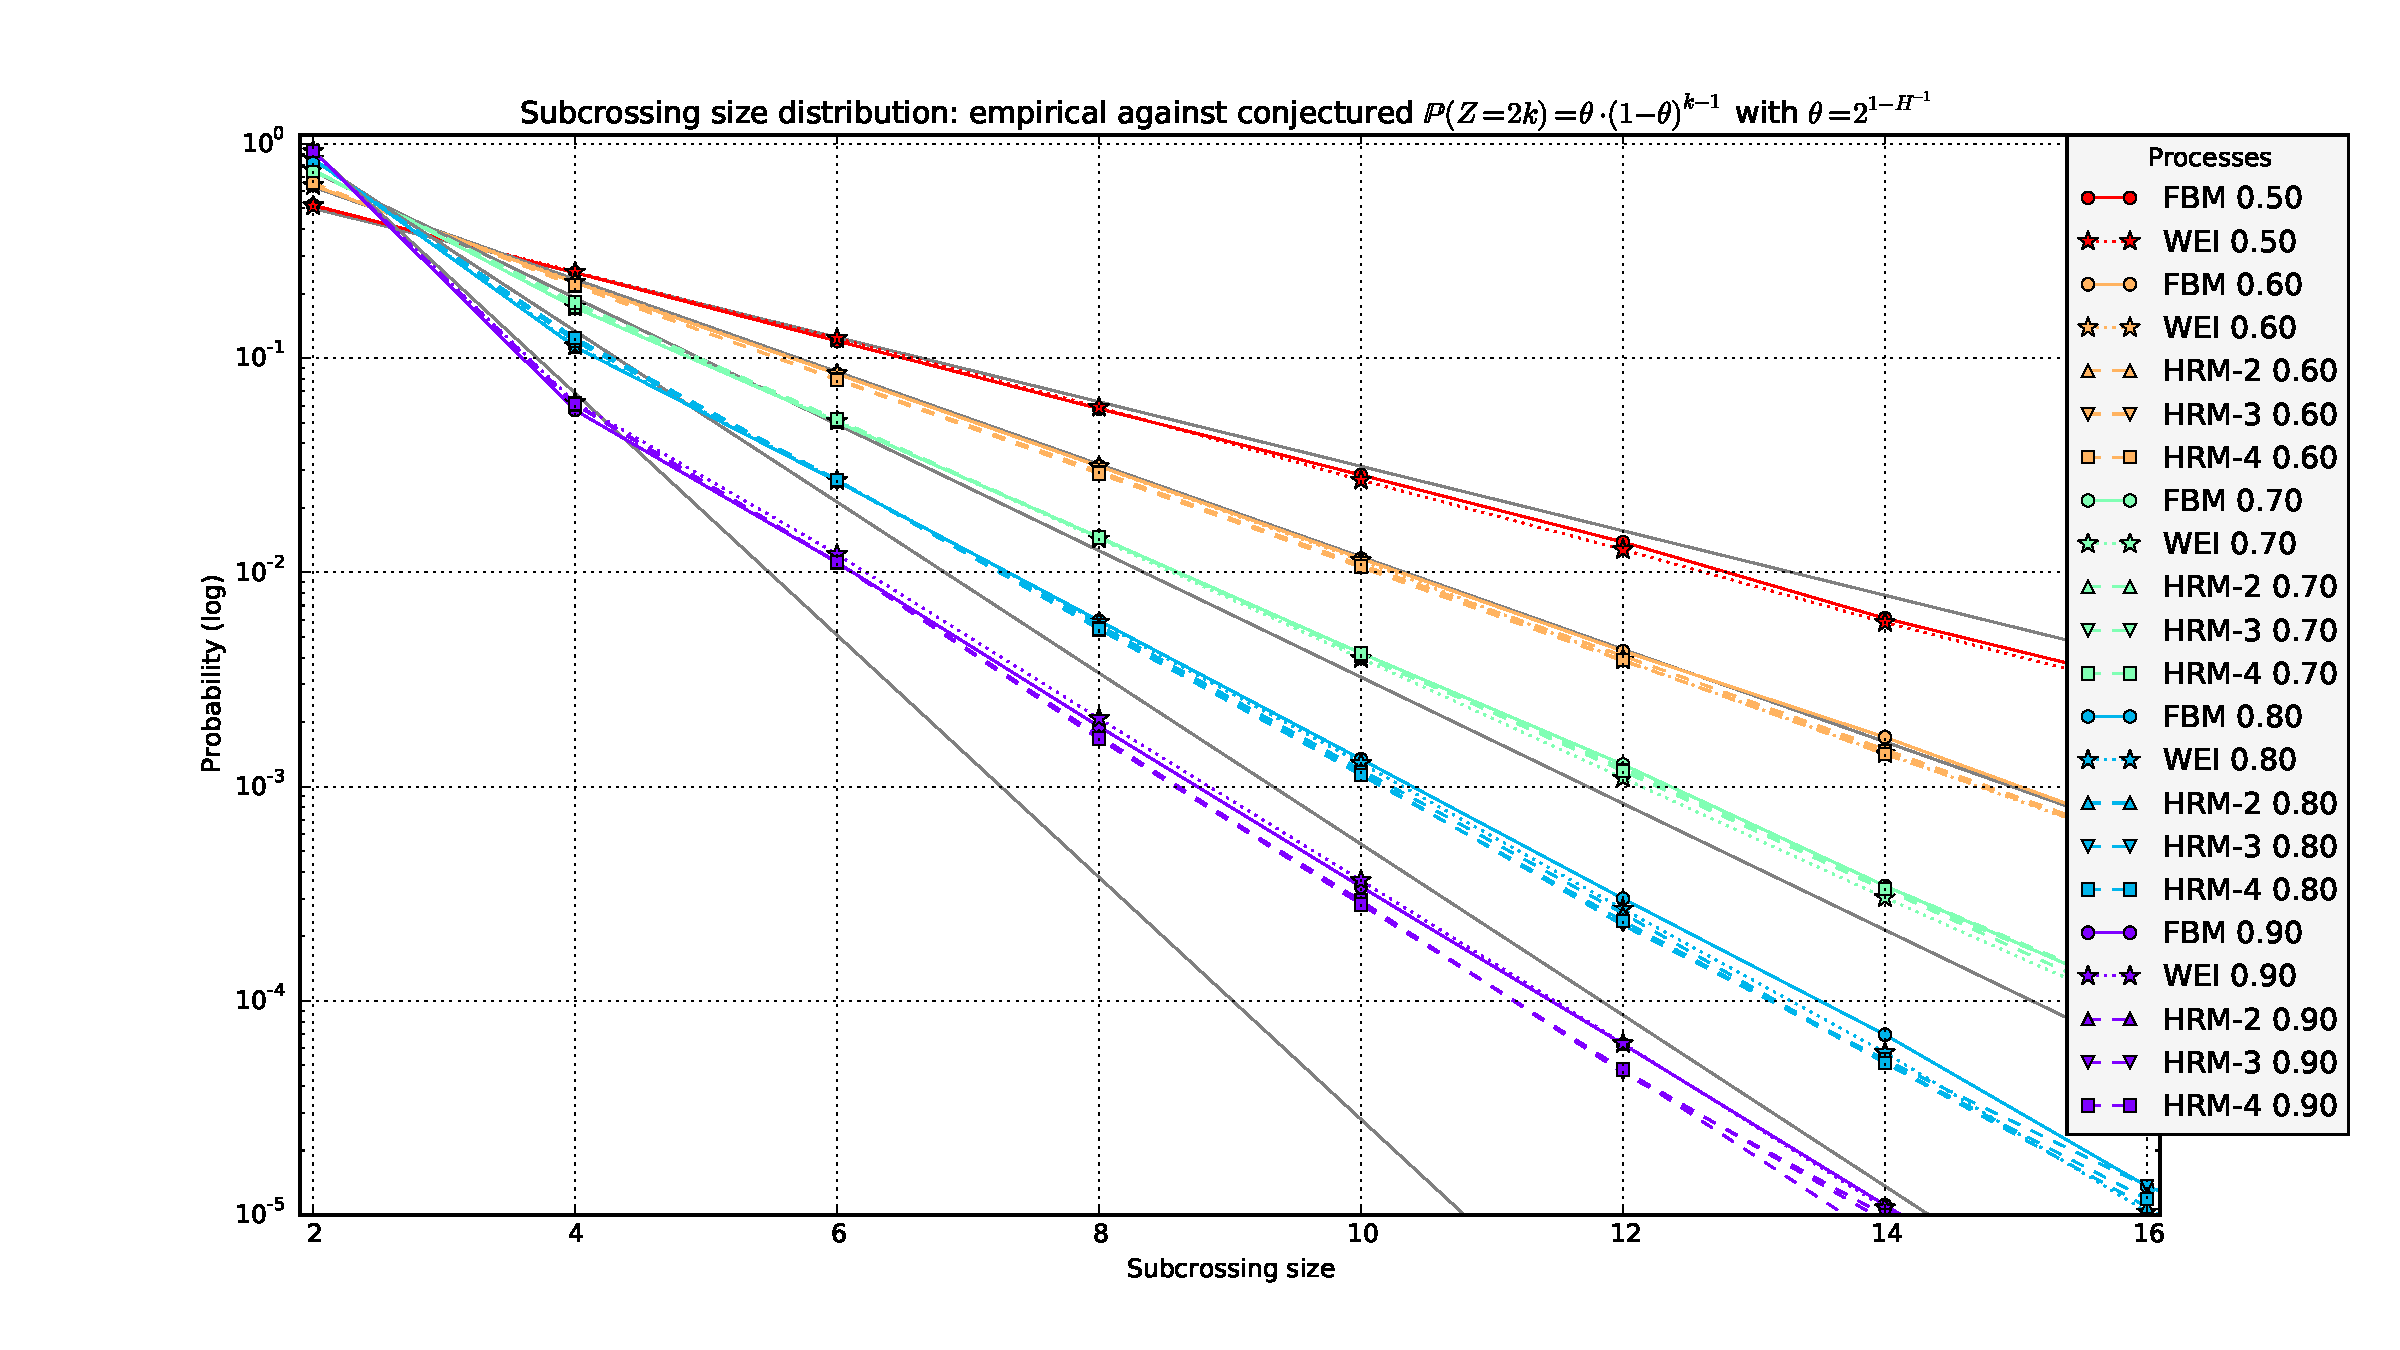
\includegraphics[width=6in]{images/fig_02_med_10000-17}
    \caption{Empirical probabilities of the crossing sizes against the hypothesized
    theoretical probabilities for $10^4$ sample paths of length $2^{17}$ points.}
\label{fig:all_xing_probs}
\end{center}\end{figure}

The tables \ref{tbl:empirical_probs_01} and \ref{tbl:empirical_probs_02} compare the 
conjectured probabilities against the empirical ones. Though there is no strong evidence
for the conjecture, one cannot say that it should be discarded. Indeed, looking at
the box-plots (\ref{fig:all_offspring_down_up} and \ref{fig:all_offspring_up_down})
of the conditional distribution of excursions, it is possible to see that even
though there is significant margin of error there the probabilities seem to agree
quite well with the hypothesised distribution.
\begin{table}[h]\begin{center}
	\begin{tabular}{l||l|l|l|l|}
					$H=0.6$ & $Z_k = 2$ & $Z_k = 4$ & $Z_k = 6$ & $Z_k = 8$ \\ \hline\hline
	\multirow{2}{*}{fBm} 	& $0.630$ & $0.233$ & $0.086$ & $0.032$ \\ \cline{2-5}
							& $0.644\pm0.033$ & $0.224\pm0.027$ & $0.083\pm0.017$ & $0.031\pm0.011$ \\ \hline\hline
	\multirow{2}{*}{WEI} 	& $0.630$ & $0.233$ & $0.086$ & $0.032$ \\ \cline{2-5}
							& $0.642\pm0.027$ & $0.226\pm0.026$ & $0.084\pm0.017$ & $0.031\pm0.010$ \\ \hline\hline
	\multirow{2}{*}{HRM-2} 	& $0.630$ & $0.233$ & $0.086$ & $0.032$ \\ \cline{2-5}
							& $0.663\pm0.034$ & $0.215\pm0.026$ & $0.078\pm0.015$ & $0.028\pm0.009$ \\ \hline\hline
	\multirow{2}{*}{HRM-3} 	& $0.630$ & $0.233$ & $0.086$ & $0.032$ \\ \cline{2-5}
							& $0.666\pm0.038$ & $0.214\pm0.026$ & $0.076\pm0.015$ & $0.027\pm0.009$ \\ \hline\hline
	\multirow{2}{*}{HRM-4} 	& $0.630$ & $0.233$ & $0.086$ & $0.032$ \\ \cline{2-5}
							& $0.667\pm0.039$ & $0.215\pm0.025$ & $0.076\pm0.016$ & $0.027\pm0.009$ \\ \hline\hline
	\end{tabular}
	\caption{The table of empirical probabilities of the first four values of the number
	of subcrossings in a parent crossing for $H$-sssi processes with $H=0.6$. Levels from
	6 to 8 were pooled to get the estimates.}
\label{tbl:empirical_probs_01}
\end{center}\end{table}

\begin{table}[h]\begin{center}
	\begin{tabular}{l||l|l|l|l|}
					$H=0.8$ & $Z_k = 2$ & $Z_k = 4$ & $Z_k = 6$ & $Z_k = 8$ \\ \hline\hline
	\multirow{2}{*}{fBm} 	& $0.841$ & $0.134$ & $0.021$ & $0.003$ \\ \cline{2-5}
 							& $0.855\pm0.023$ & $0.112\pm0.017$ & $0.026\pm0.006$ & $0.006\pm0.002$ \\ \hline\hline
	\multirow{2}{*}{HRM-2} 	& $0.841$ & $0.134$ & $0.021$ & $0.003$ \\ \cline{2-5}
 							& $0.848\pm0.027$ & $0.118\pm0.022$ & $0.026\pm0.006$ & $0.005\pm0.002$ \\ \hline\hline
	\multirow{2}{*}{HRM-3} 	& $0.841$ & $0.134$ & $0.021$ & $0.003$ \\ \cline{2-5}
 							& $0.846\pm0.024$ & $0.121\pm0.019$ & $0.026\pm0.006$ & $0.005\pm0.002$ \\ \hline\hline
	\multirow{2}{*}{HRM-4} 	& $0.841$ & $0.134$ & $0.021$ & $0.003$ \\ \cline{2-5}
 							& $0.844\pm0.021$ & $0.122\pm0.016$ & $0.026\pm0.006$ & $0.005\pm0.002$ \\ \hline\hline
	\multirow{2}{*}{WEI} 	& $0.841$ & $0.134$ & $0.021$ & $0.003$ \\ \cline{2-5}
 							& $0.854\pm0.019$ & $0.113\pm0.015$ & $0.026\pm0.005$ & $0.006\pm0.002$ \\ \hline\hline
	\end{tabular}
	\caption{The table of empirical probabilities of the first four values of the number
	of subcrossings in a parent crossing for $H$-sssi processes with $H=0.8$. Levels from
	6 to 8 were pooled to get the estimates.}
\label{tbl:empirical_probs_02}
\end{center}\end{table}

Crossing duration also do not seem contradict the hypothesized scaling for $H$-sssi
processes and the Weierstrass function (see fig.~\ref{fig:wei_durations} - \ref{fig:hrm_4_durations}).
Also we considered the properly scaled empirical quantiles (not presented here) of
the crossing durations between the processes considered and across all sufficiently
populated levels (from $1$-st to $10$-th) of the sample crossing tree. The conclusion
is that there is indeed similarity (up to a multiplicative constant depending on
the base scale $\delta$) of the crossing durations' distribution among processes
(see fig.~\ref{fig:fbm_quantiles_06}, \ref{fig:fbm_quantiles_08} and \ref{fig:fbm_quantiles_durations}).

\begin{figure}[htb]\begin{center}
    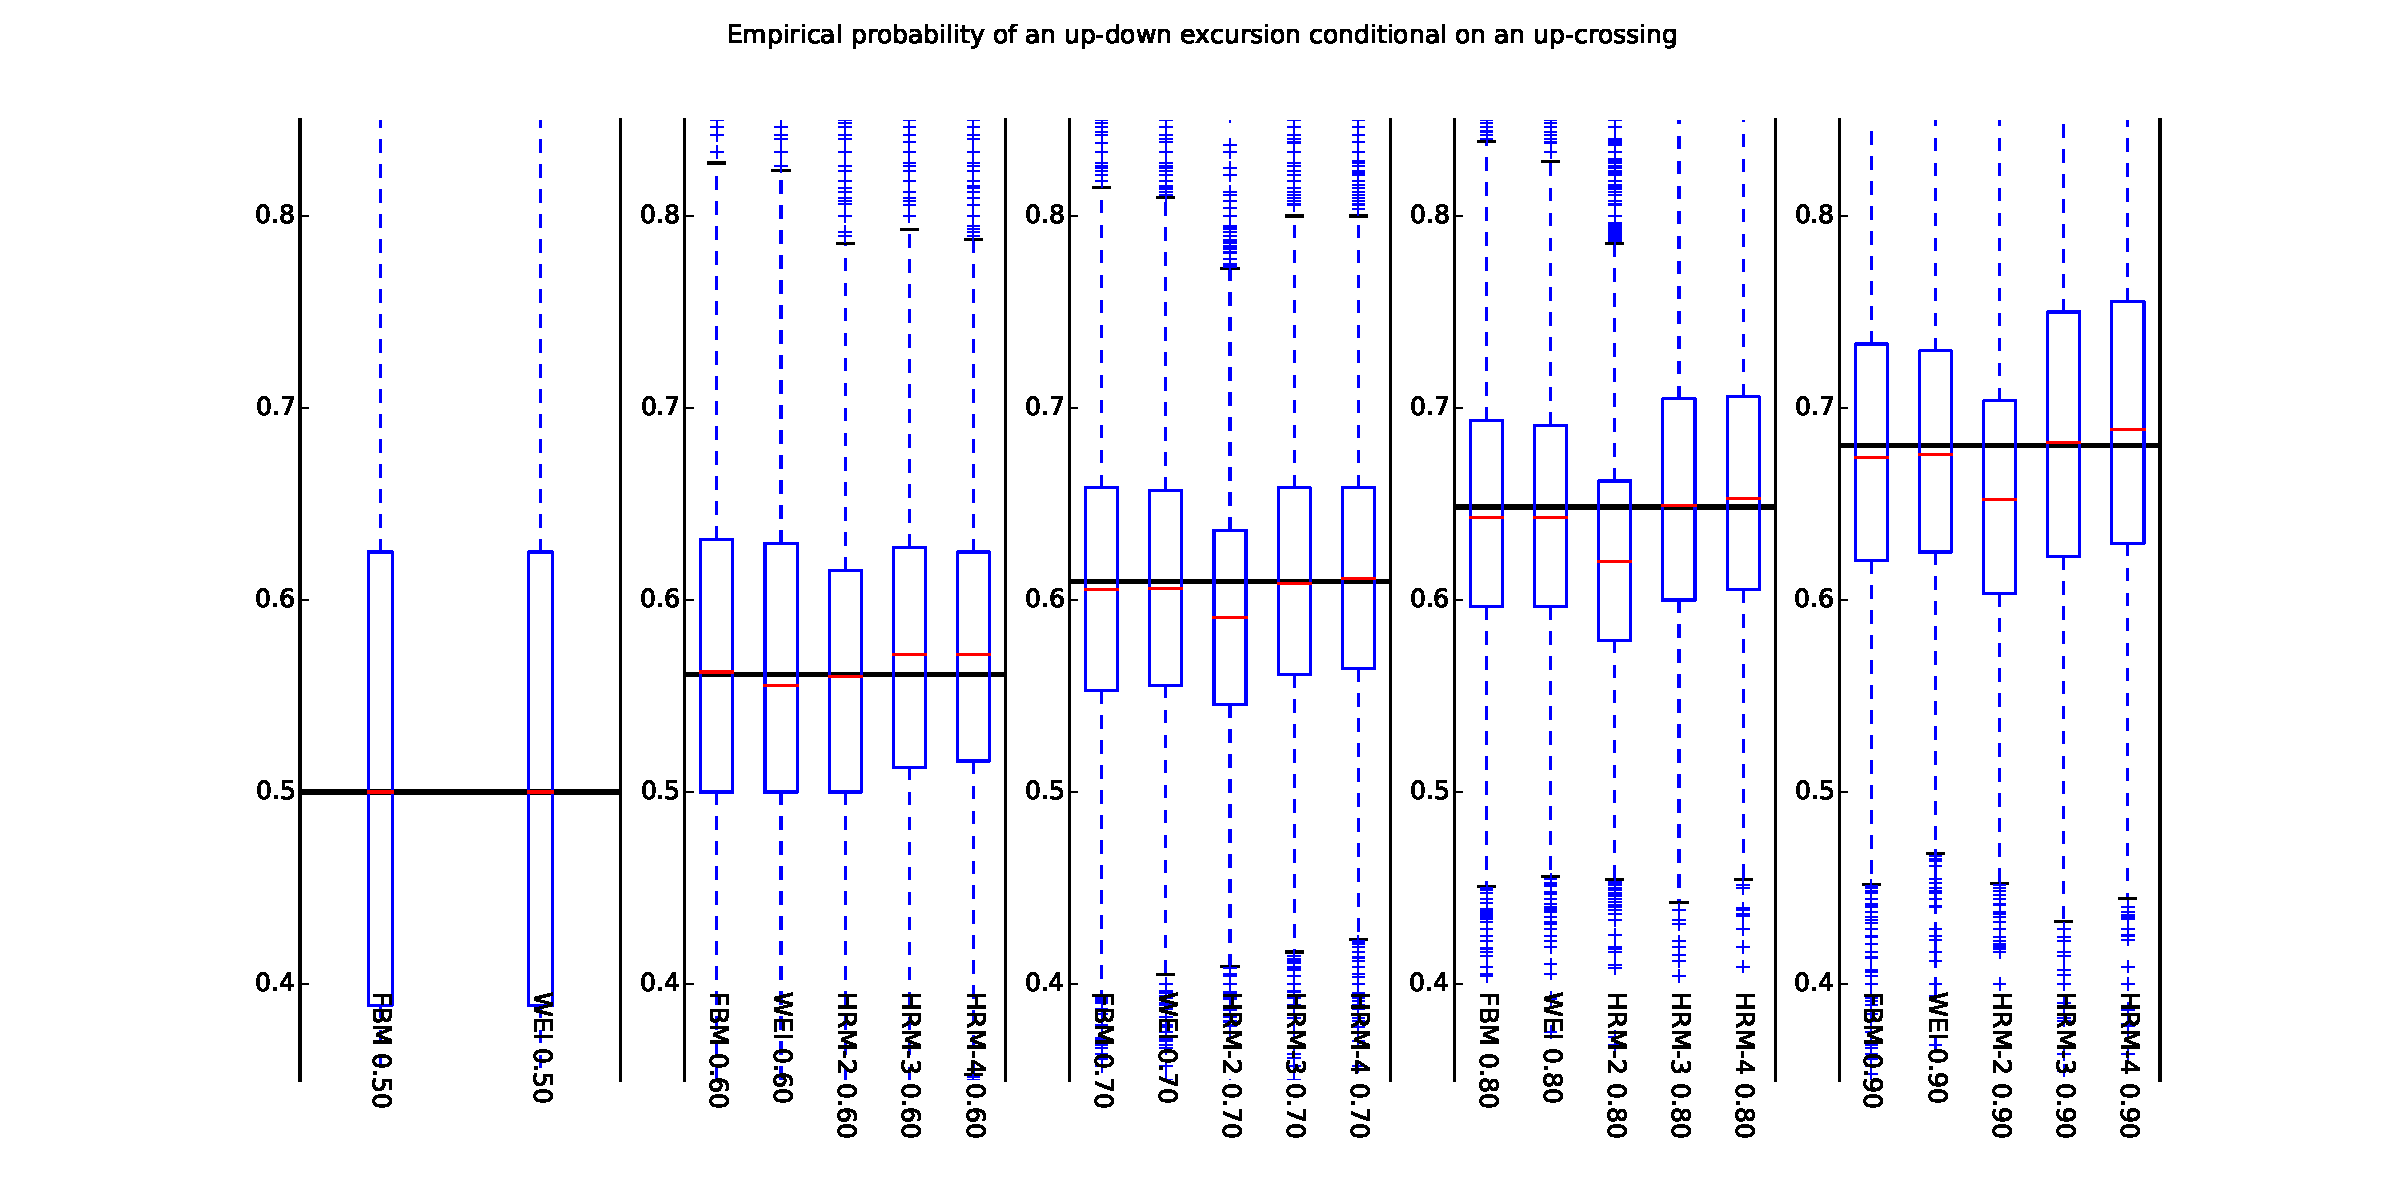
\includegraphics[width=6in]{images/fig_03_up-down_med_10000-17}
    \caption{The empirical estimates of the probability of an up-down excursion conditional on
    the upward orientation of the parent crossing.}
\label{fig:all_offspring_up_down}
\end{center}\end{figure}

\begin{figure}[htb]\begin{center}
    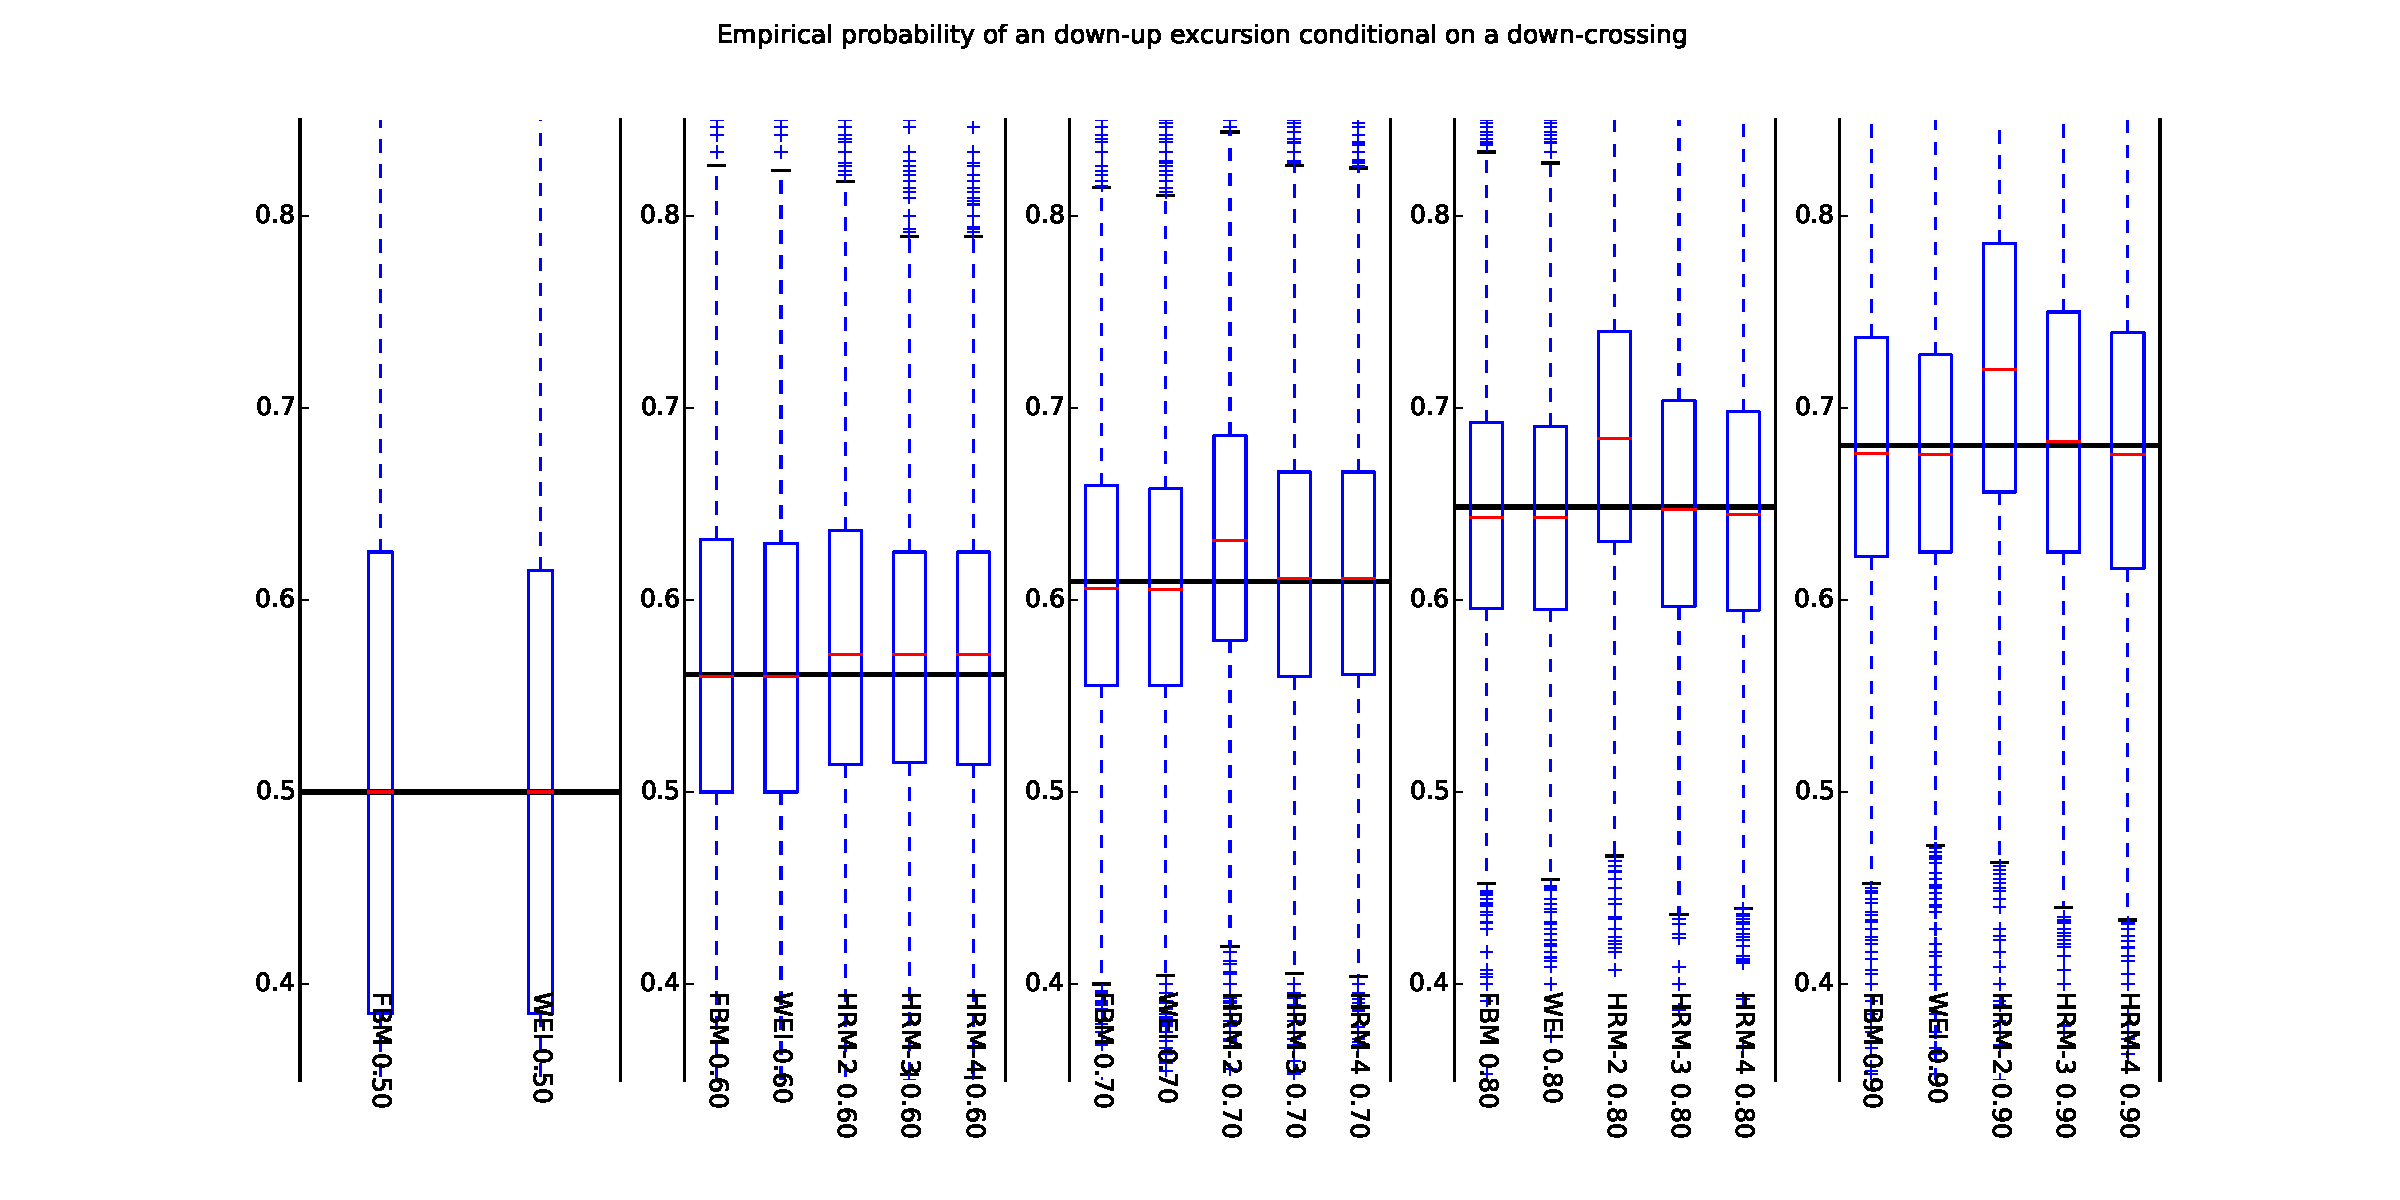
\includegraphics[width=6in]{images/fig_03_down-up_med_10000-17}
    \caption{The same figure as~\ref{fig:all_offspring_up_down} but for down-up excursions
    conditional on the orientation of the parent crossing being downward.}
\label{fig:all_offspring_down_up}
\end{center}\end{figure}

\begin{figure}[htb]\begin{center}
    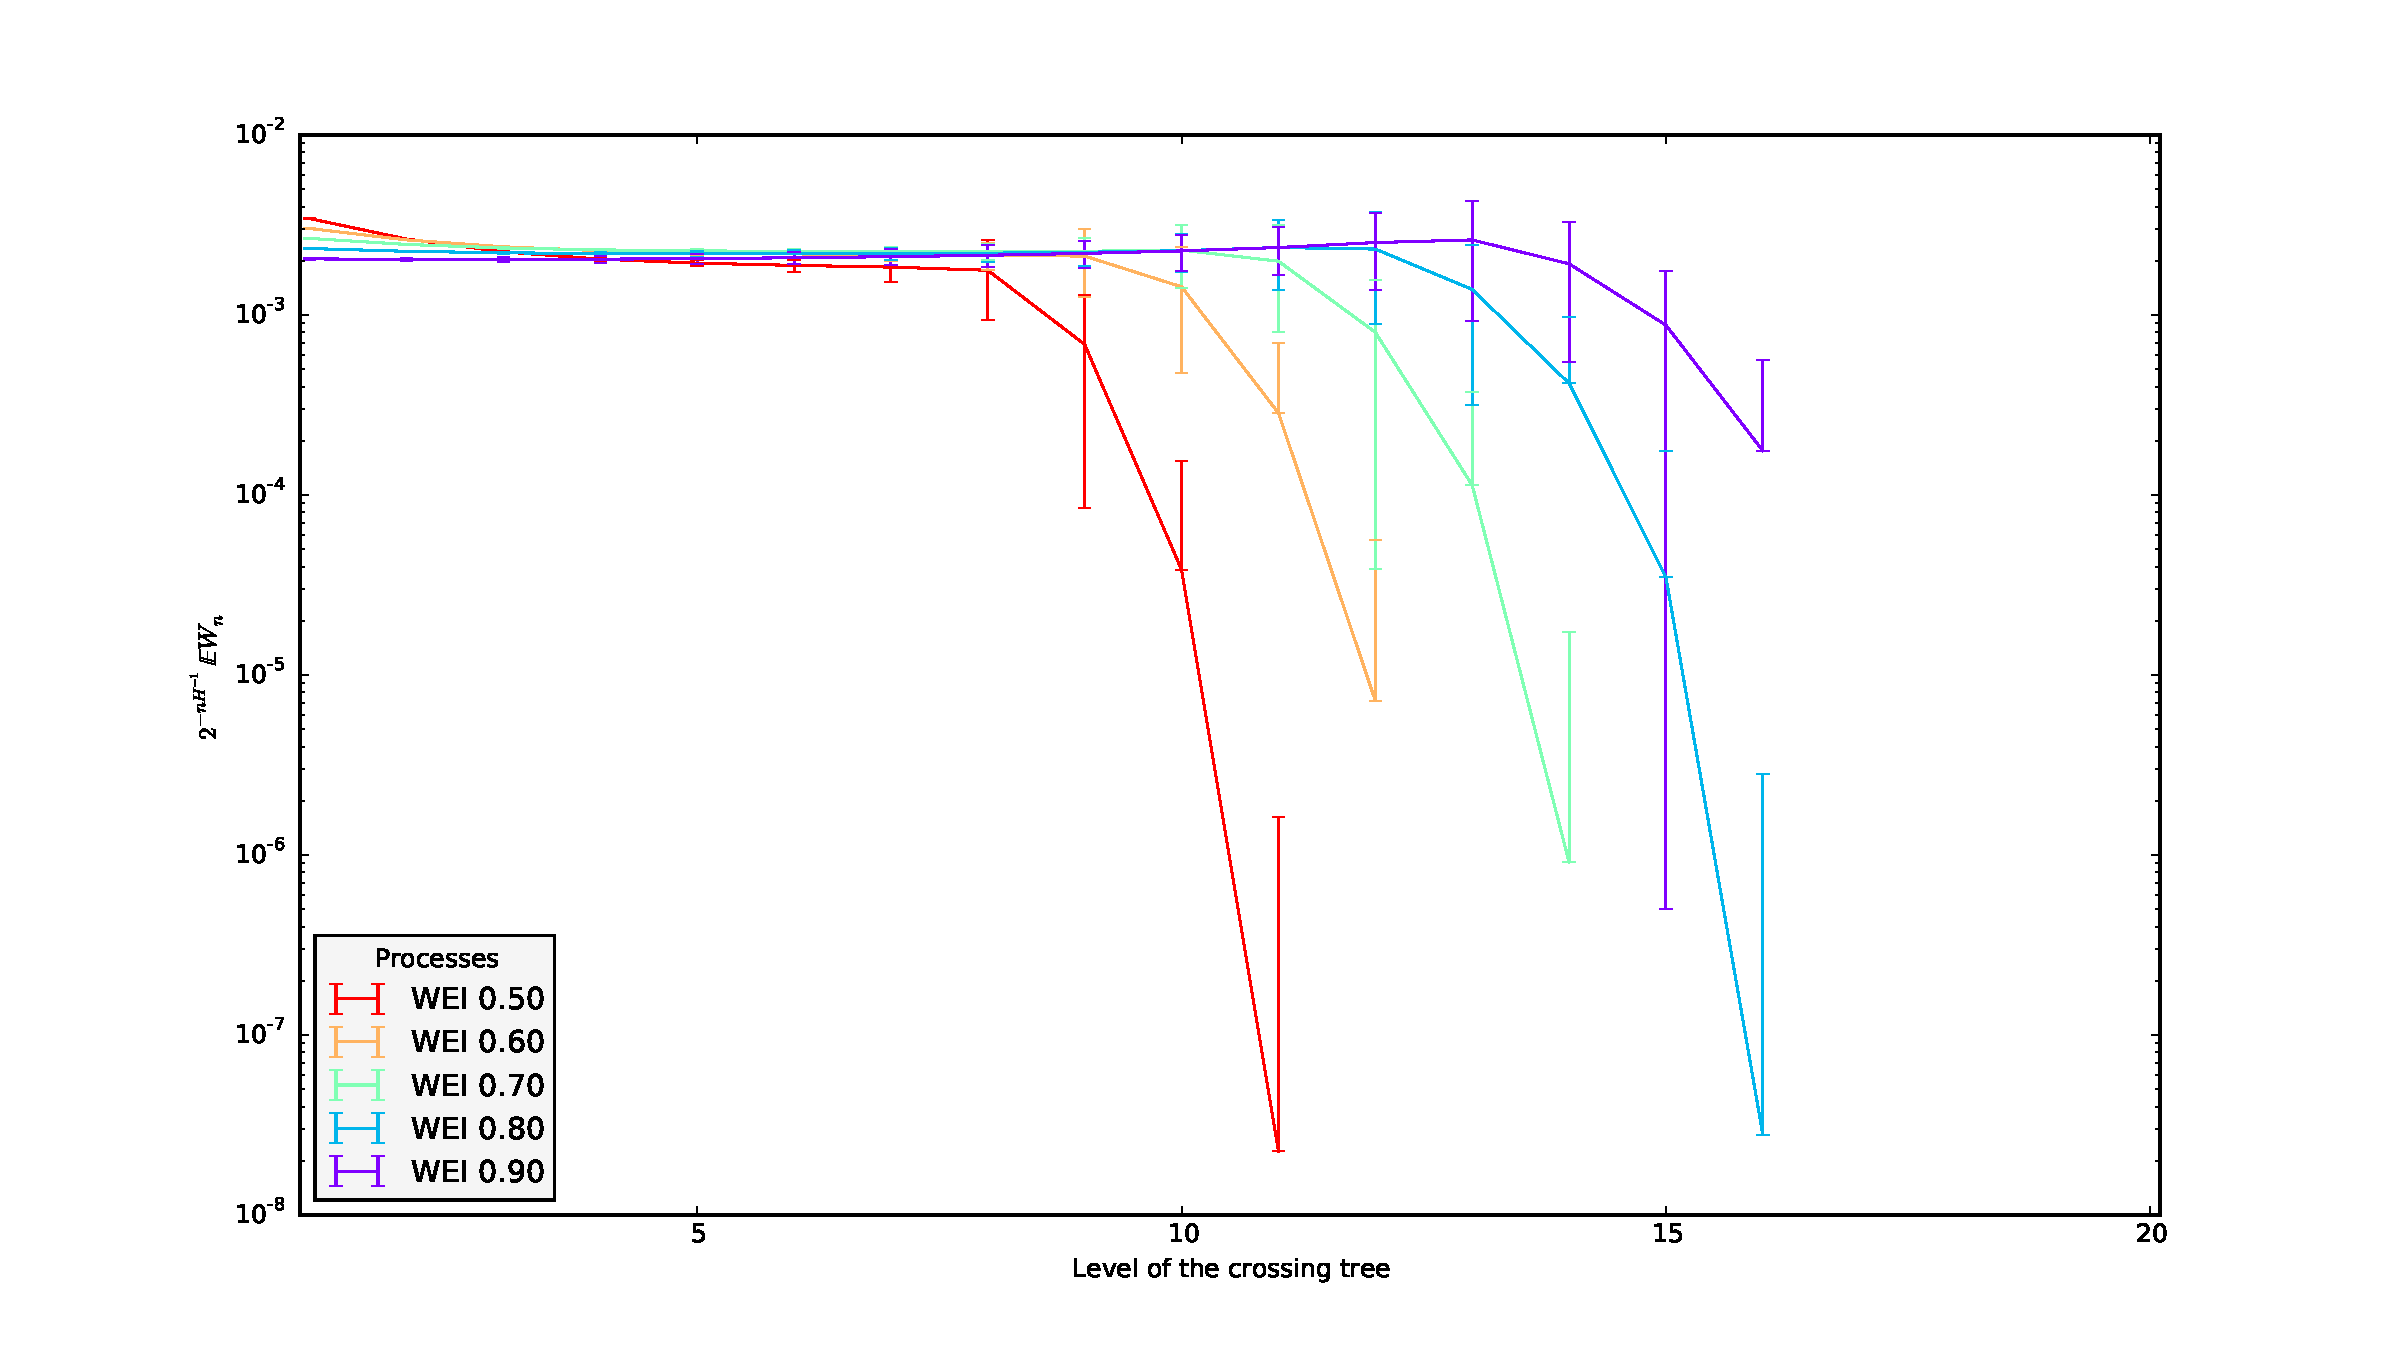
\includegraphics[width=6in]{images/fig_08_med_WEI_10000-17}
    \caption{The average crossing duration at each level of the crossing tree built
    for the Weierstrass processes.}
\label{fig:wei_durations}
\end{center}\end{figure}

\begin{figure}[htb]\begin{center}
    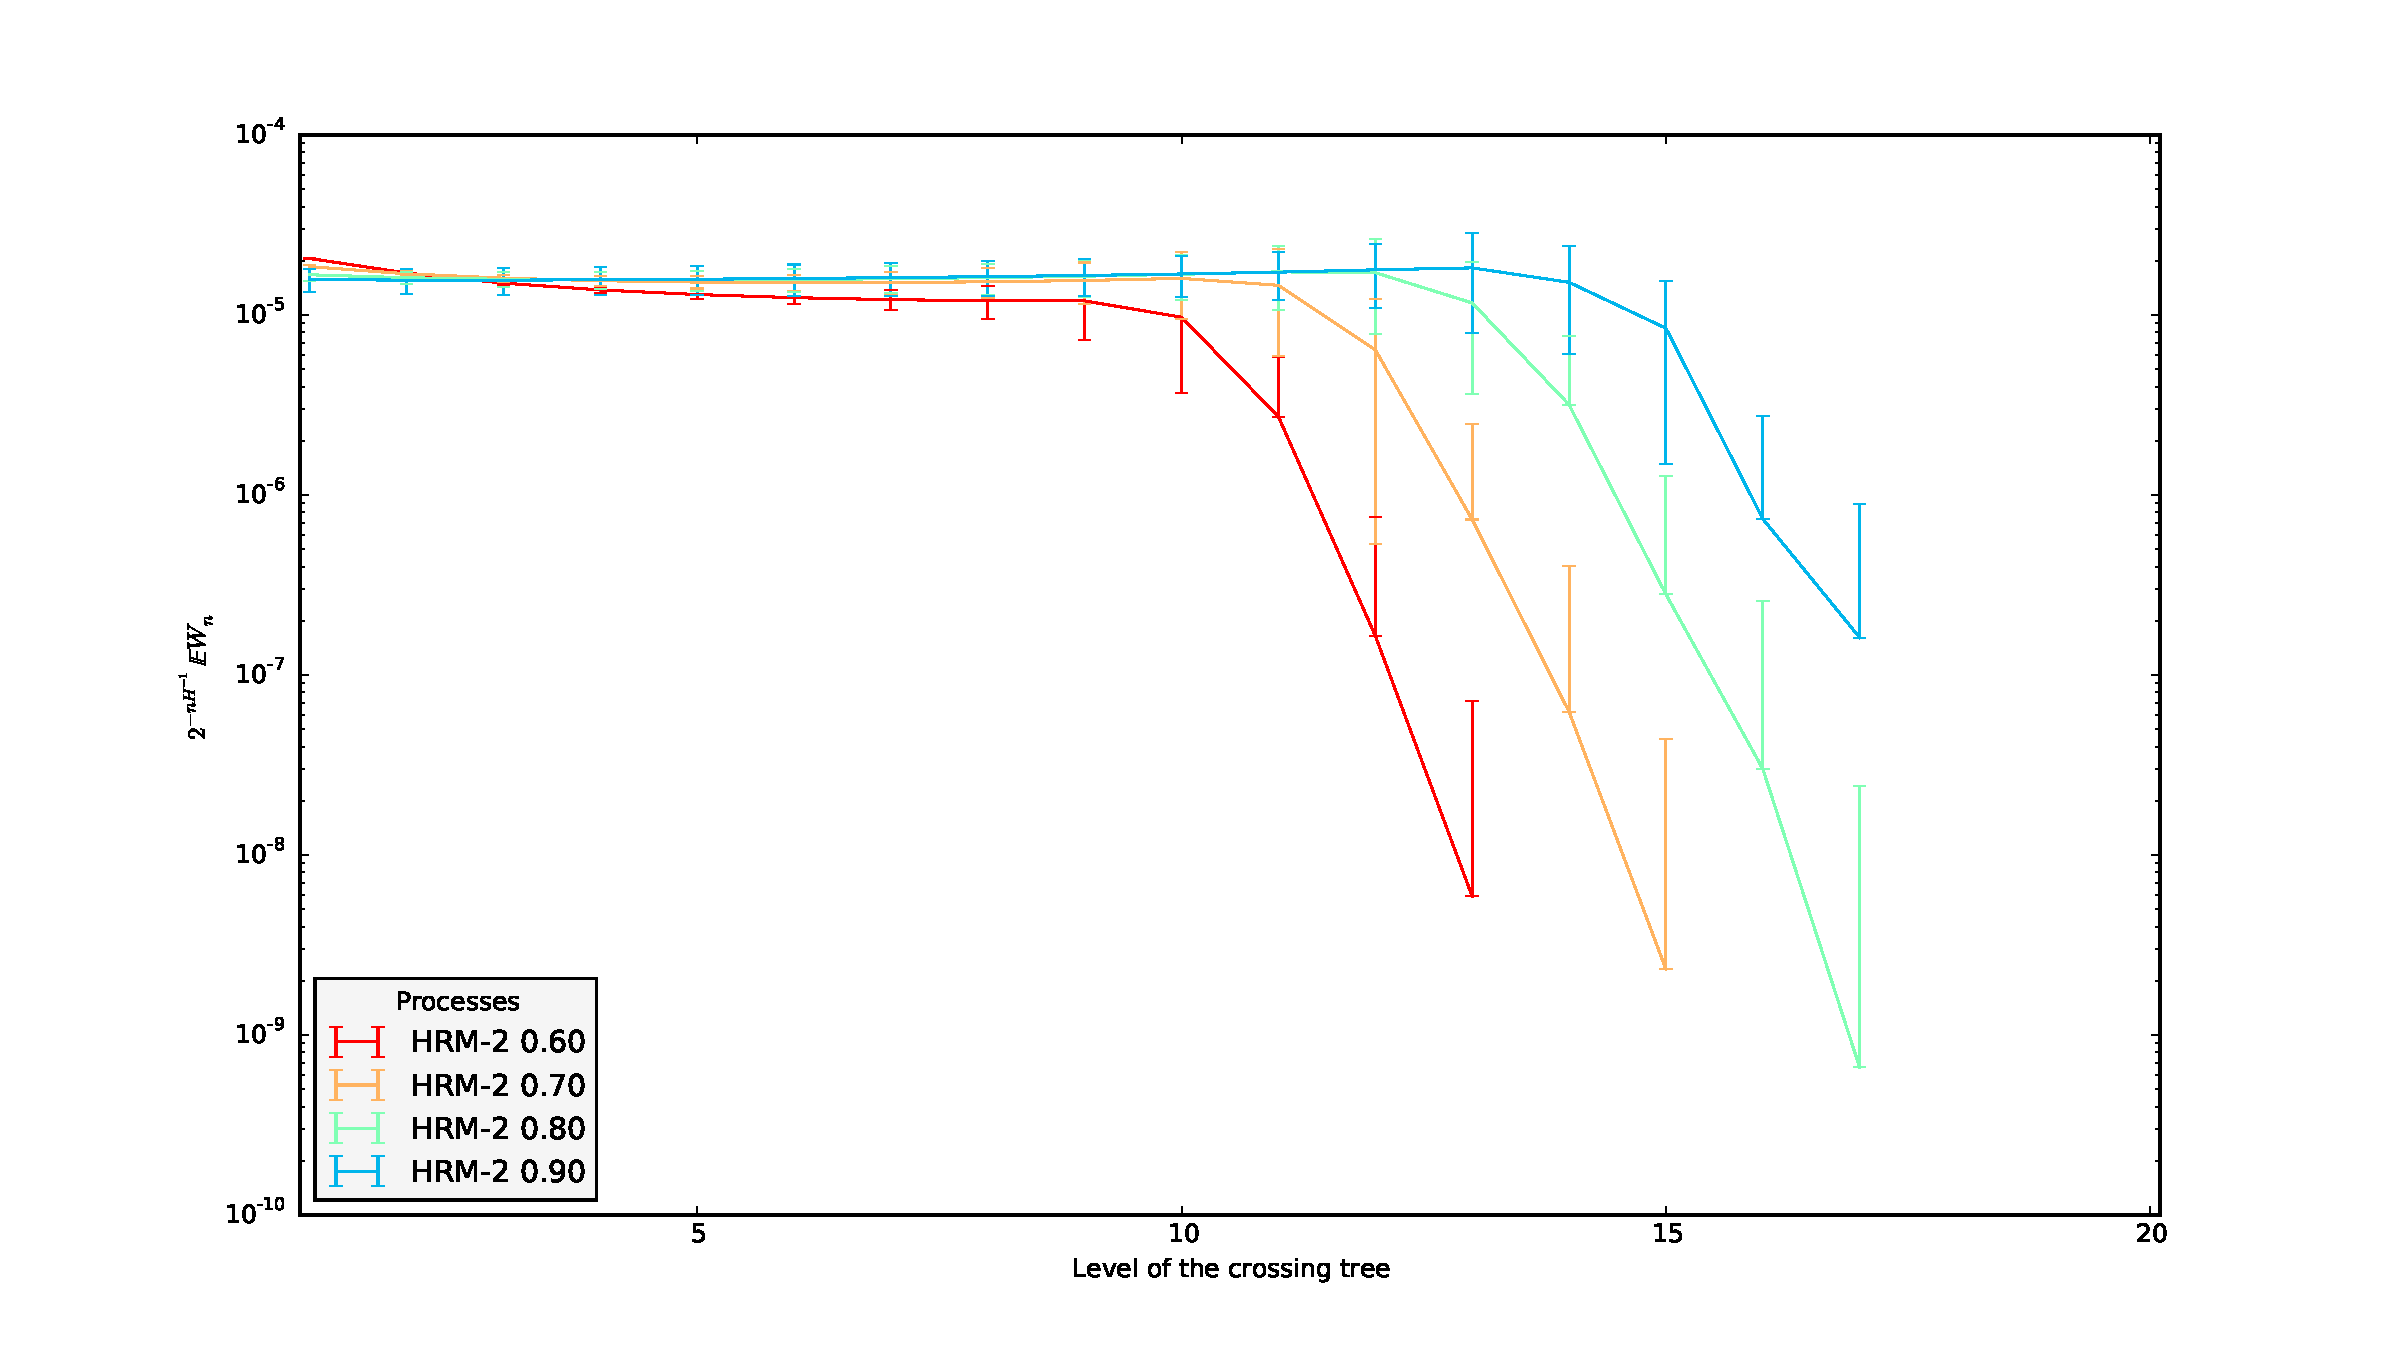
\includegraphics[width=6in]{images/fig_08_med_HRM-2_10000-17}
    \caption{The average crossing duration at each level of the crossing tree built
    for the Hermite processes of order $2$.}
\label{fig:hrm_2_durations}
\end{center}\end{figure}


\begin{figure}[htb]\begin{center}
    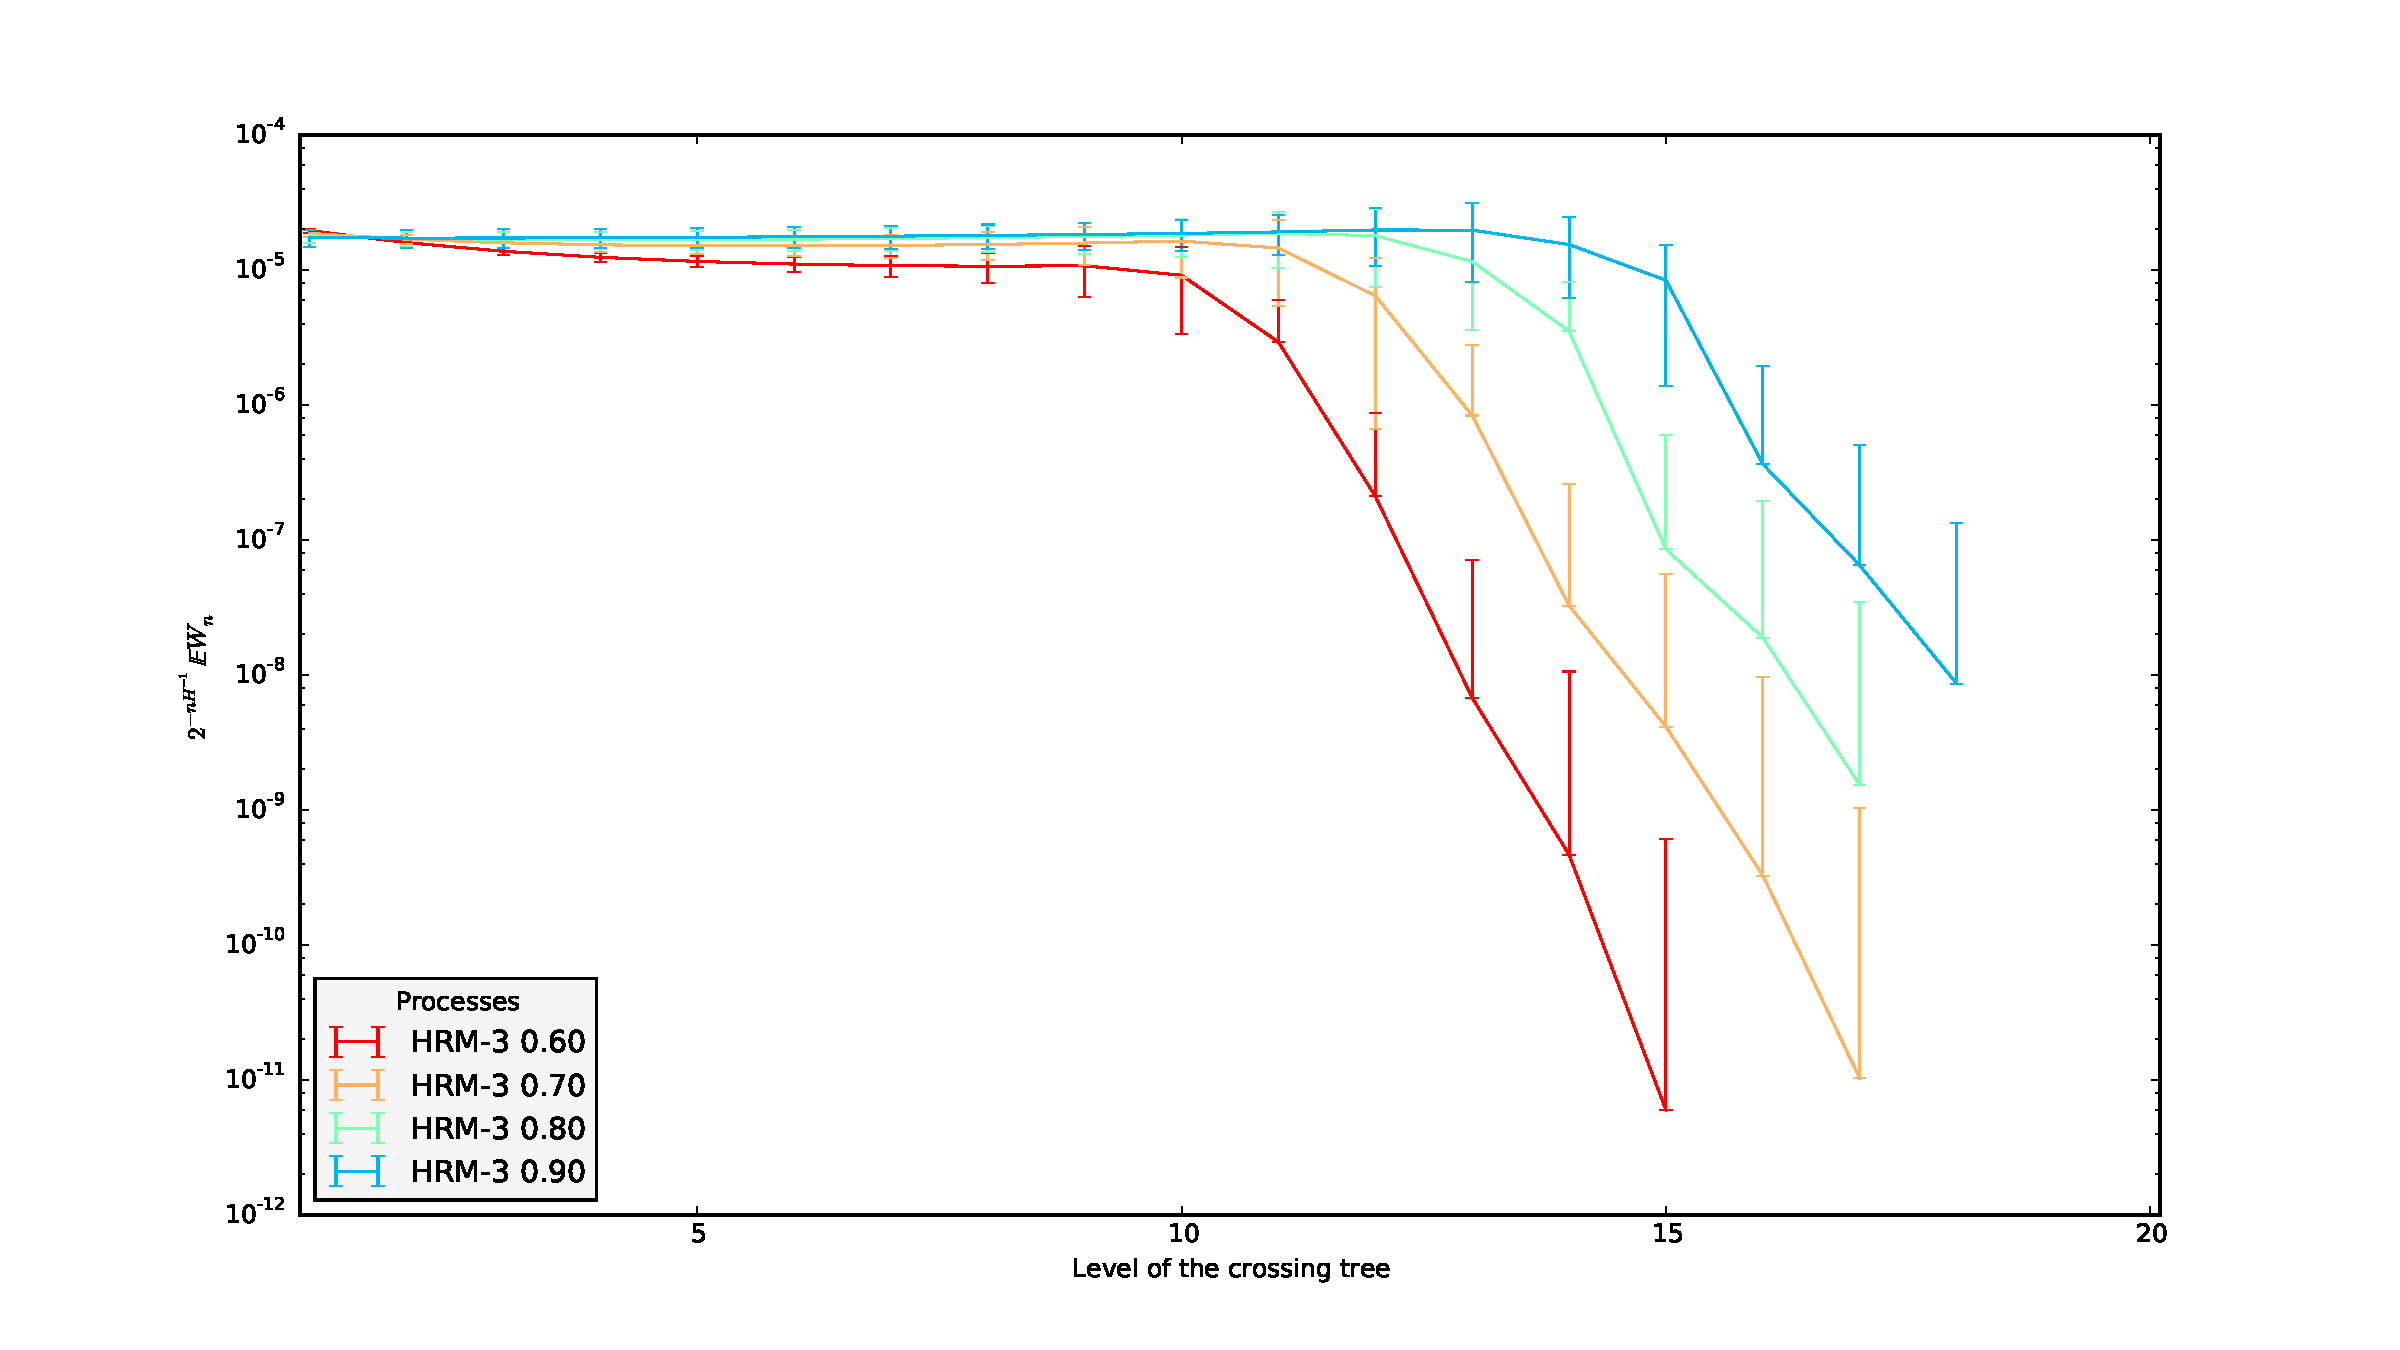
\includegraphics[width=6in]{images/fig_08_med_HRM-3_10000-17}
    \caption{The average crossing duration at each level of the crossing tree built
    for the Hermite processes of order $3$.}
\label{fig:hrm_3_durations}
\end{center}\end{figure}

\begin{figure}[htb]\begin{center}
    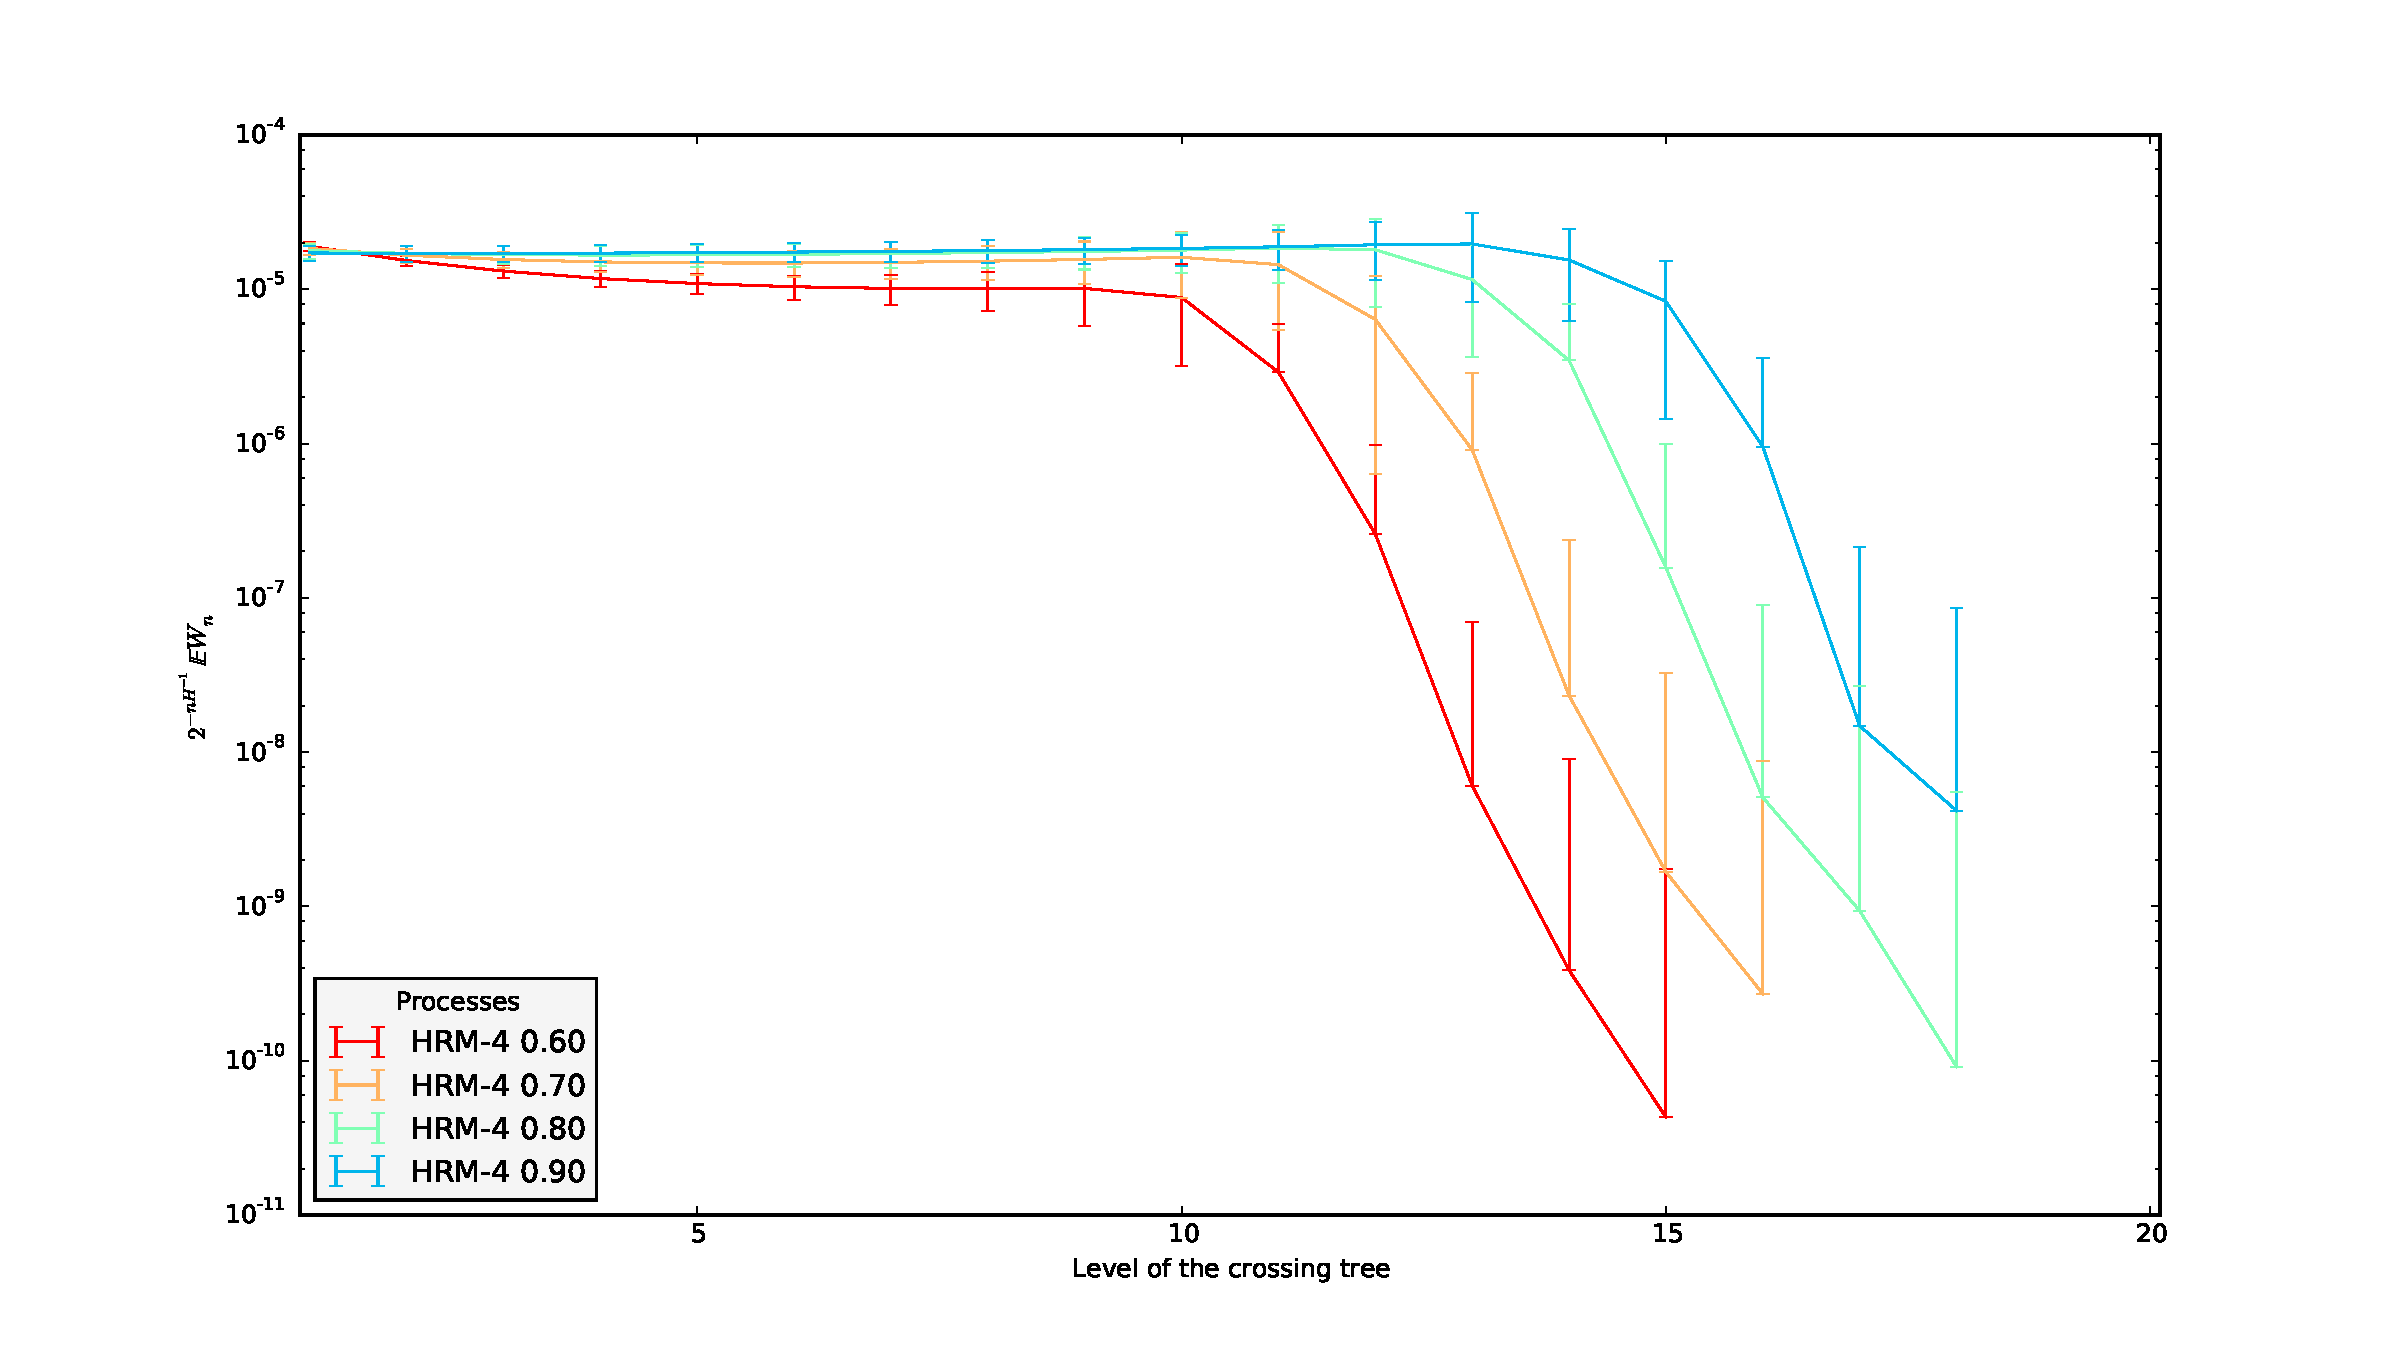
\includegraphics[width=6in]{images/fig_08_med_HRM-4_10000-17}
    \caption{The average crossing duration at each level of the crossing tree built
    for the Hermite processes of order $4$.}
\label{fig:hrm_4_durations}
\end{center}\end{figure}


\begin{figure}[htb]\begin{center}
    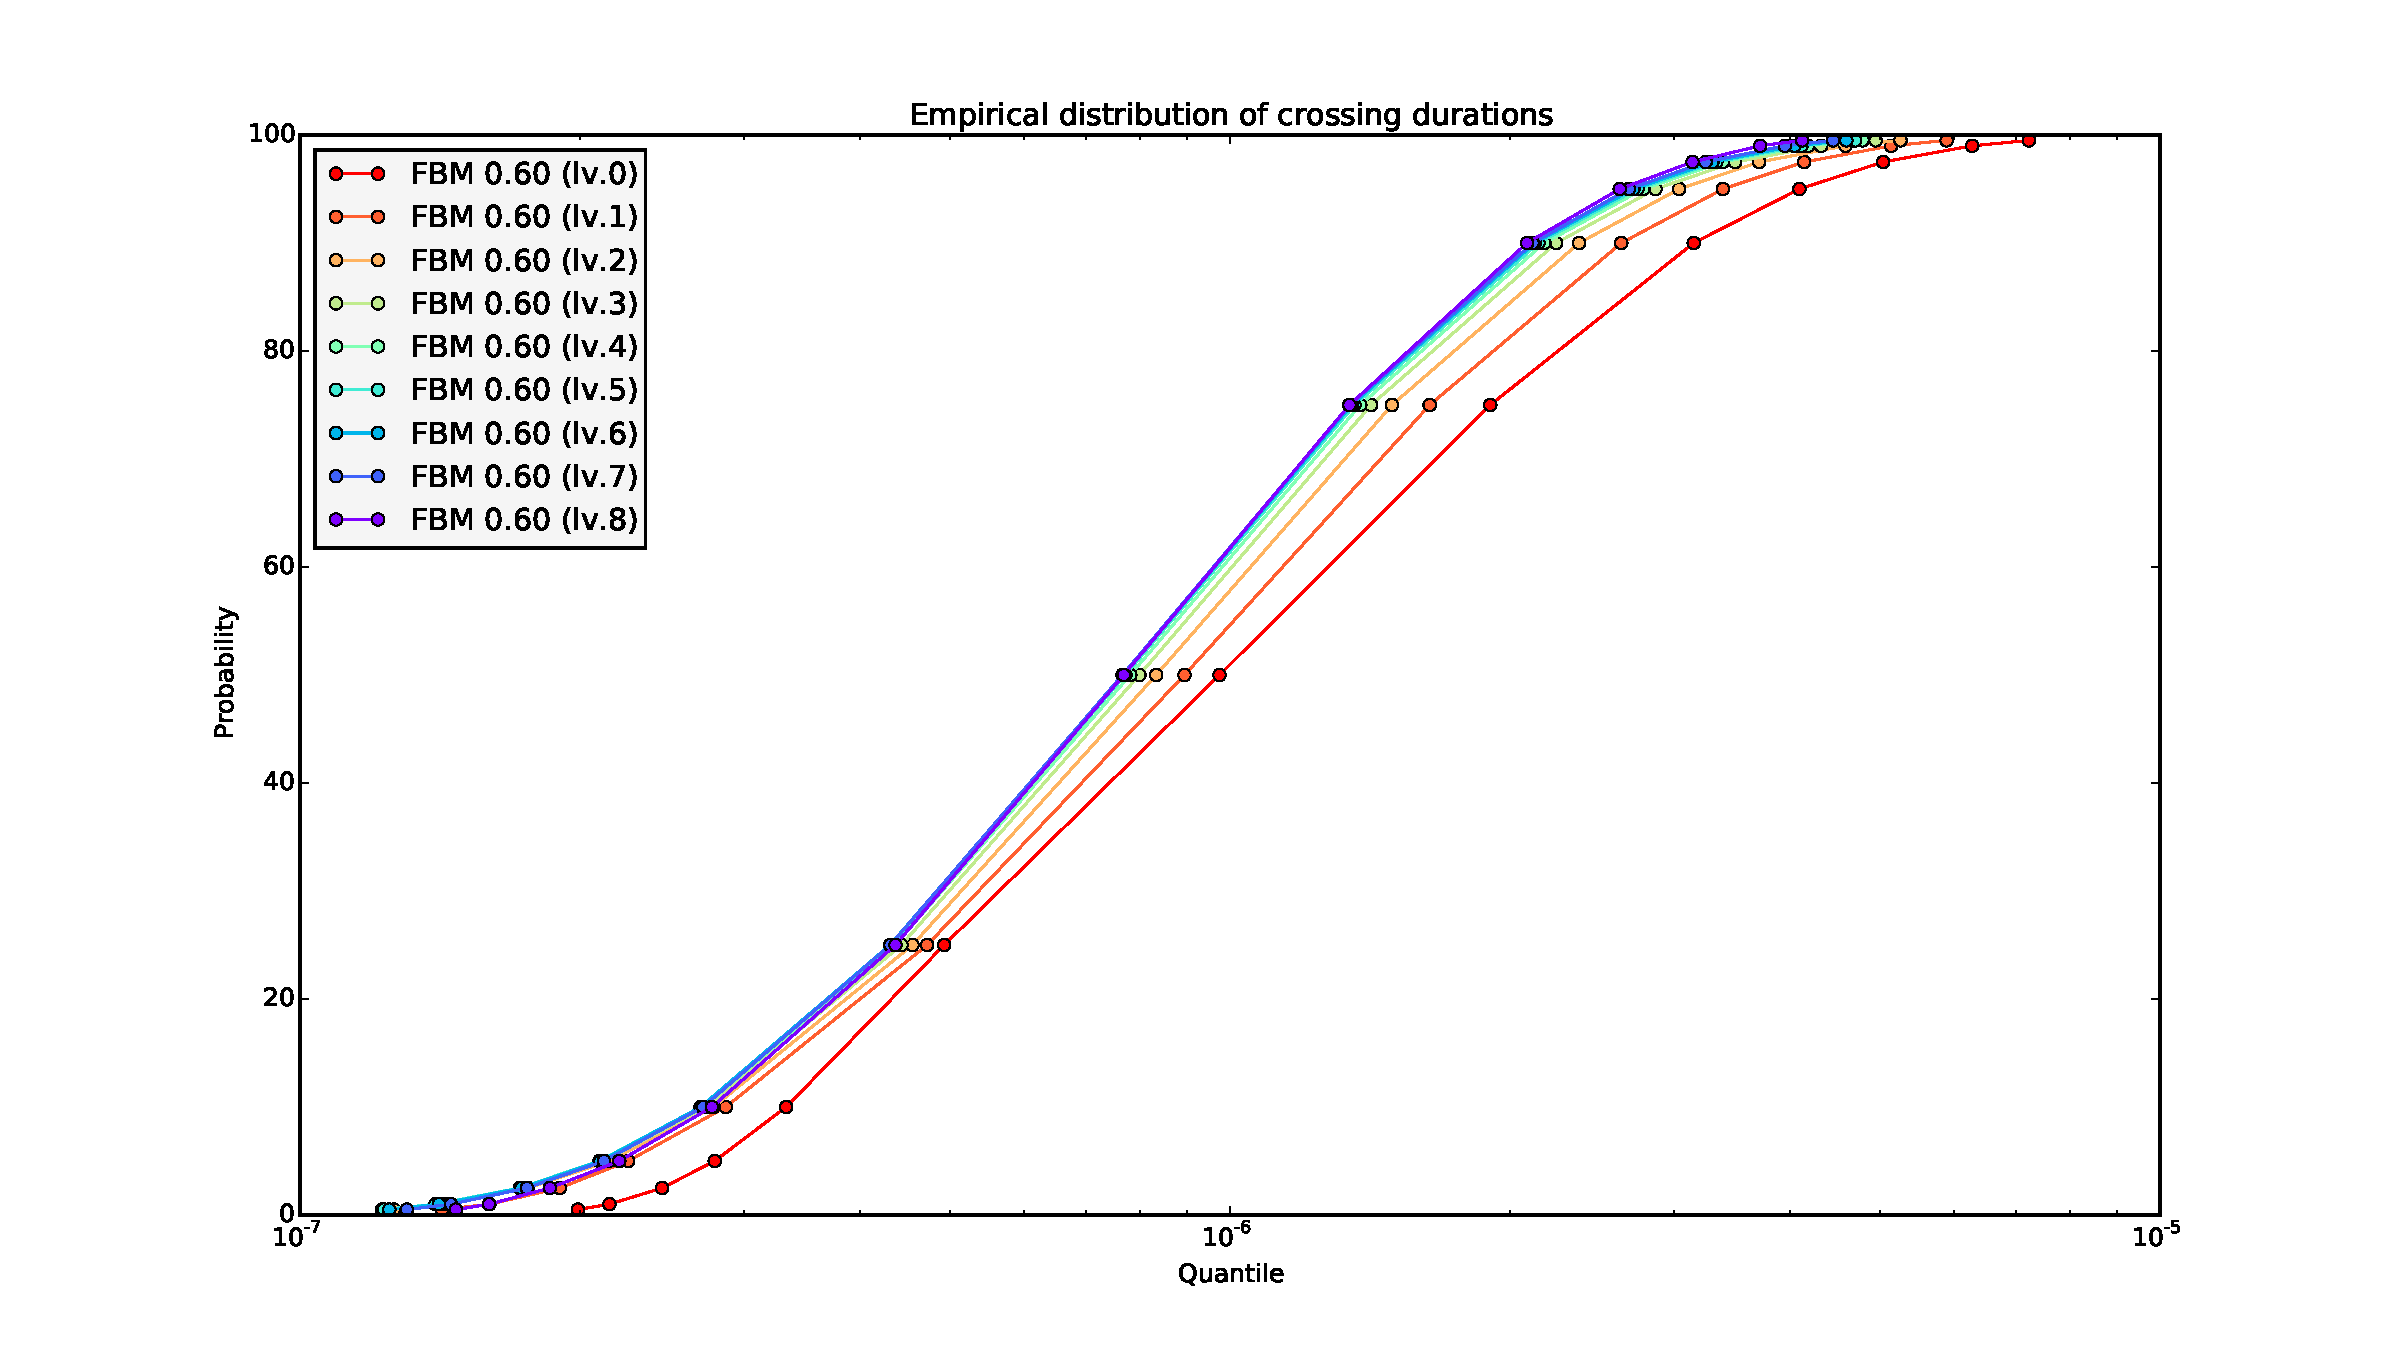
\includegraphics[width=6in]{images/fig_09_med_FBM_060}
    \caption{The empirical distribution of crossing durations at each level of the
    crossing tree built for the fractional Brownian motion ($2^{21}$ datapoints) with $H = 0.6$.
    Averaged across all Monte-Carlo realisations.}
\label{fig:fbm_quantiles_06}
\end{center}\end{figure}

\begin{figure}[htb]\begin{center}
    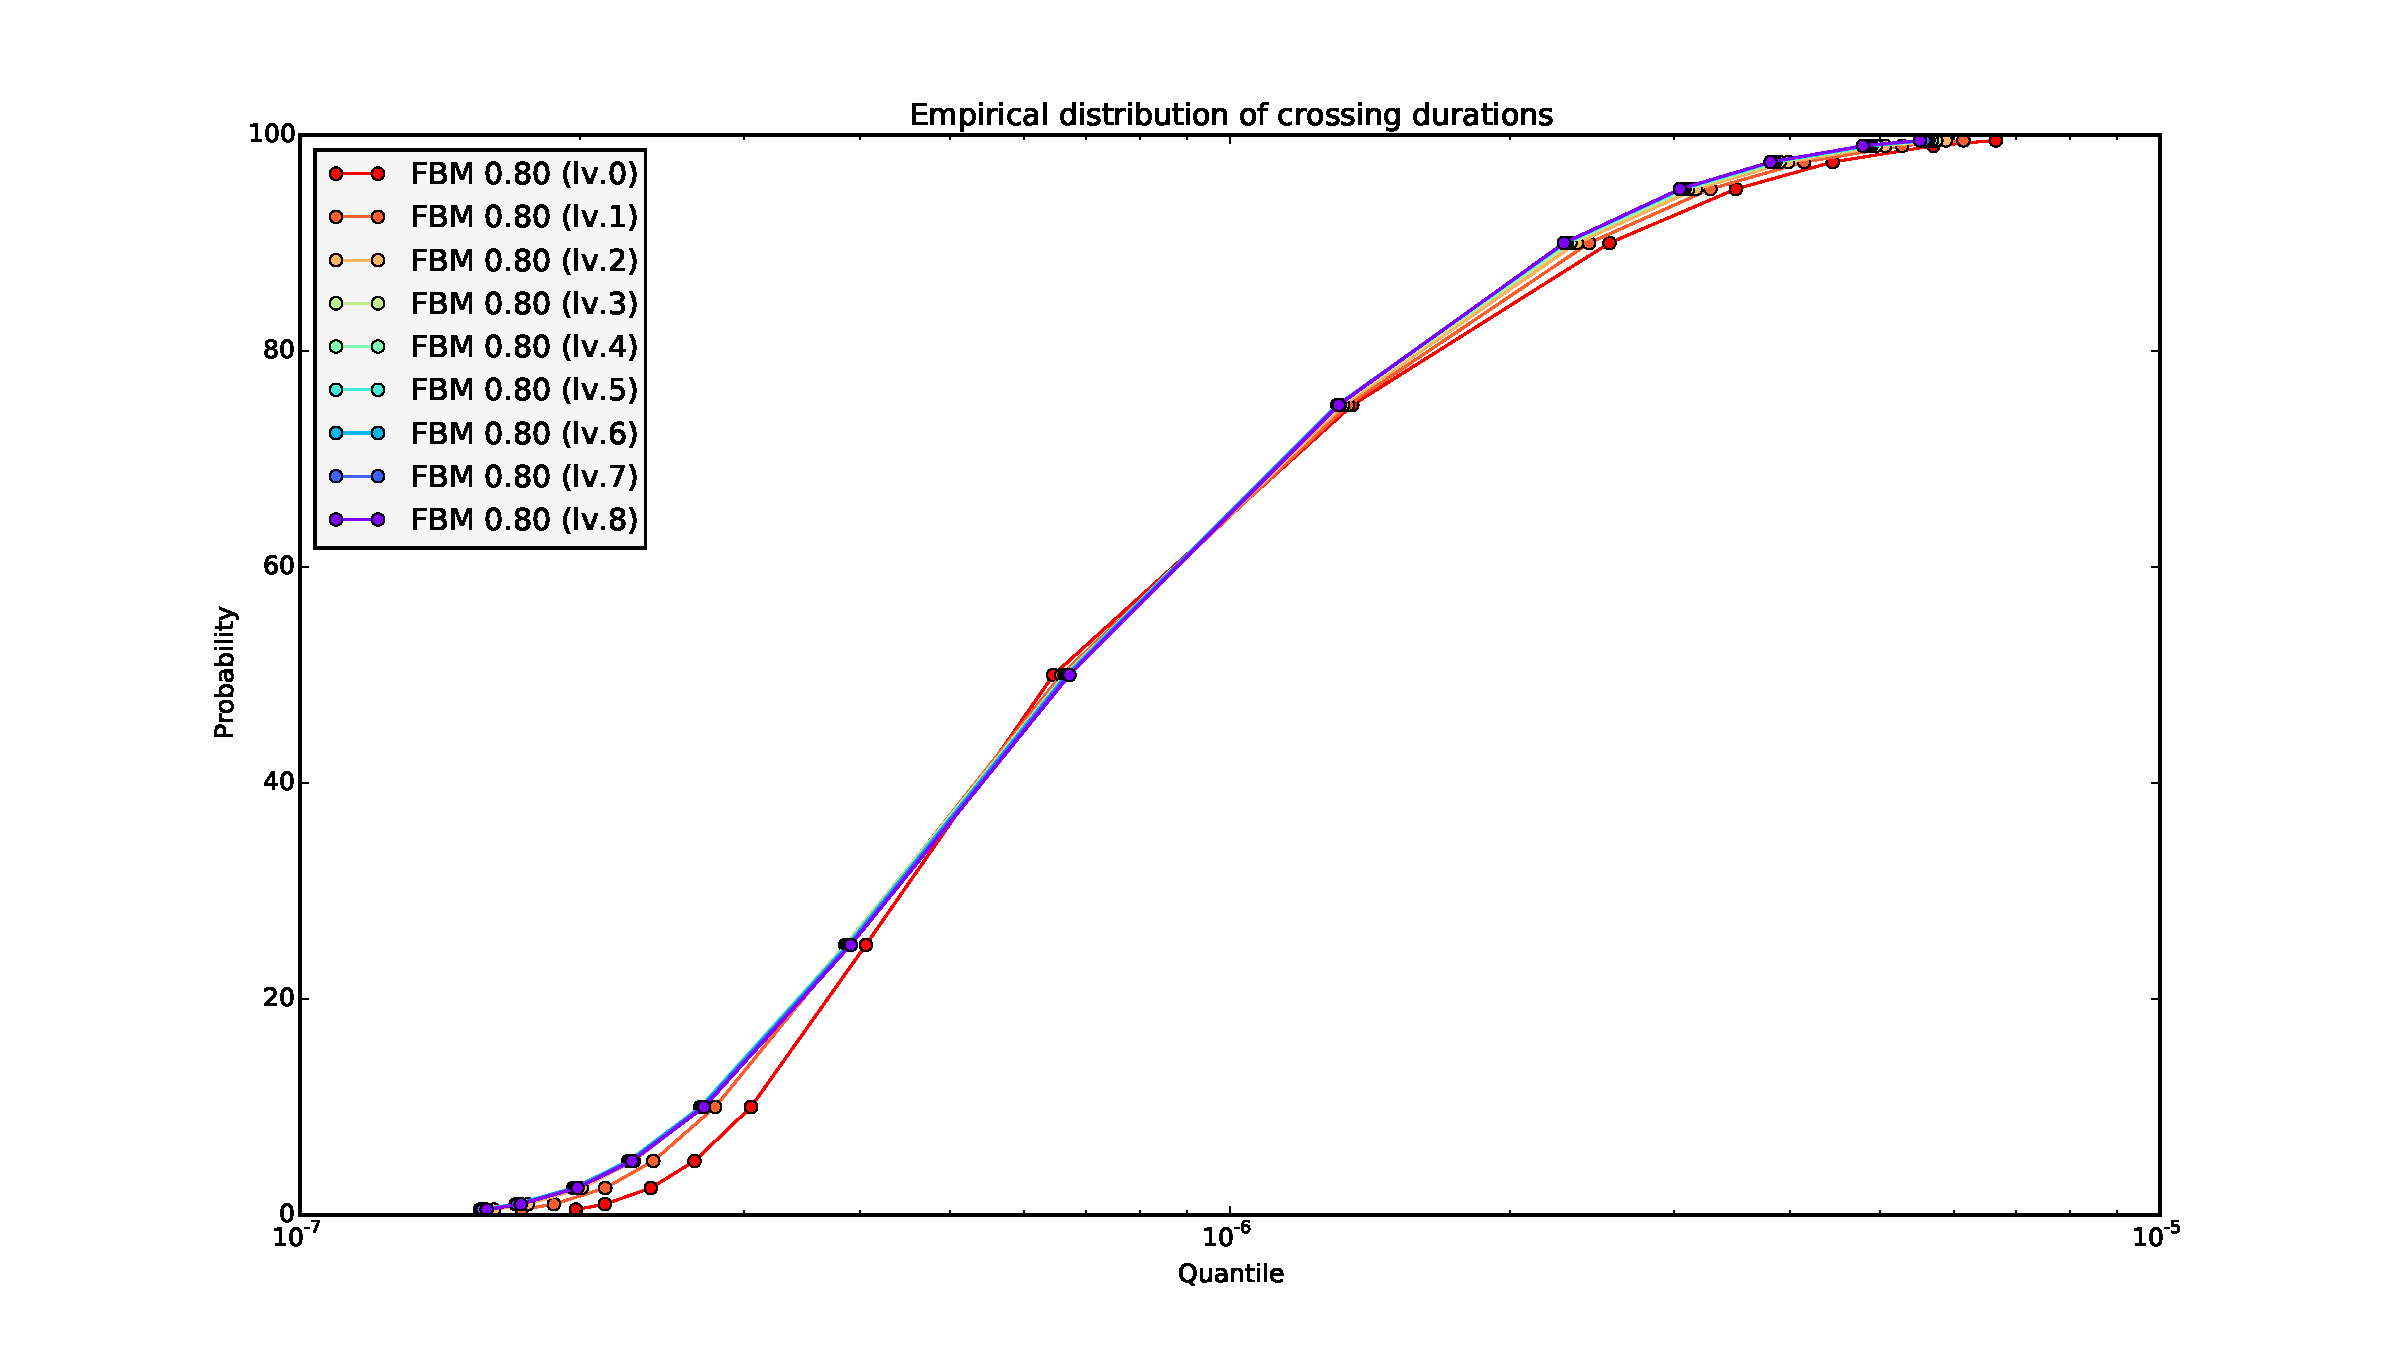
\includegraphics[width=6in]{images/fig_09_med_FBM_080}
    \caption{Similarly to figure~\ref{fig:fbm_quantiles_06} but for fBm with $H=0.8$.}
\label{fig:fbm_quantiles_08}
\end{center}\end{figure}

\begin{figure}[htb]\begin{center}
    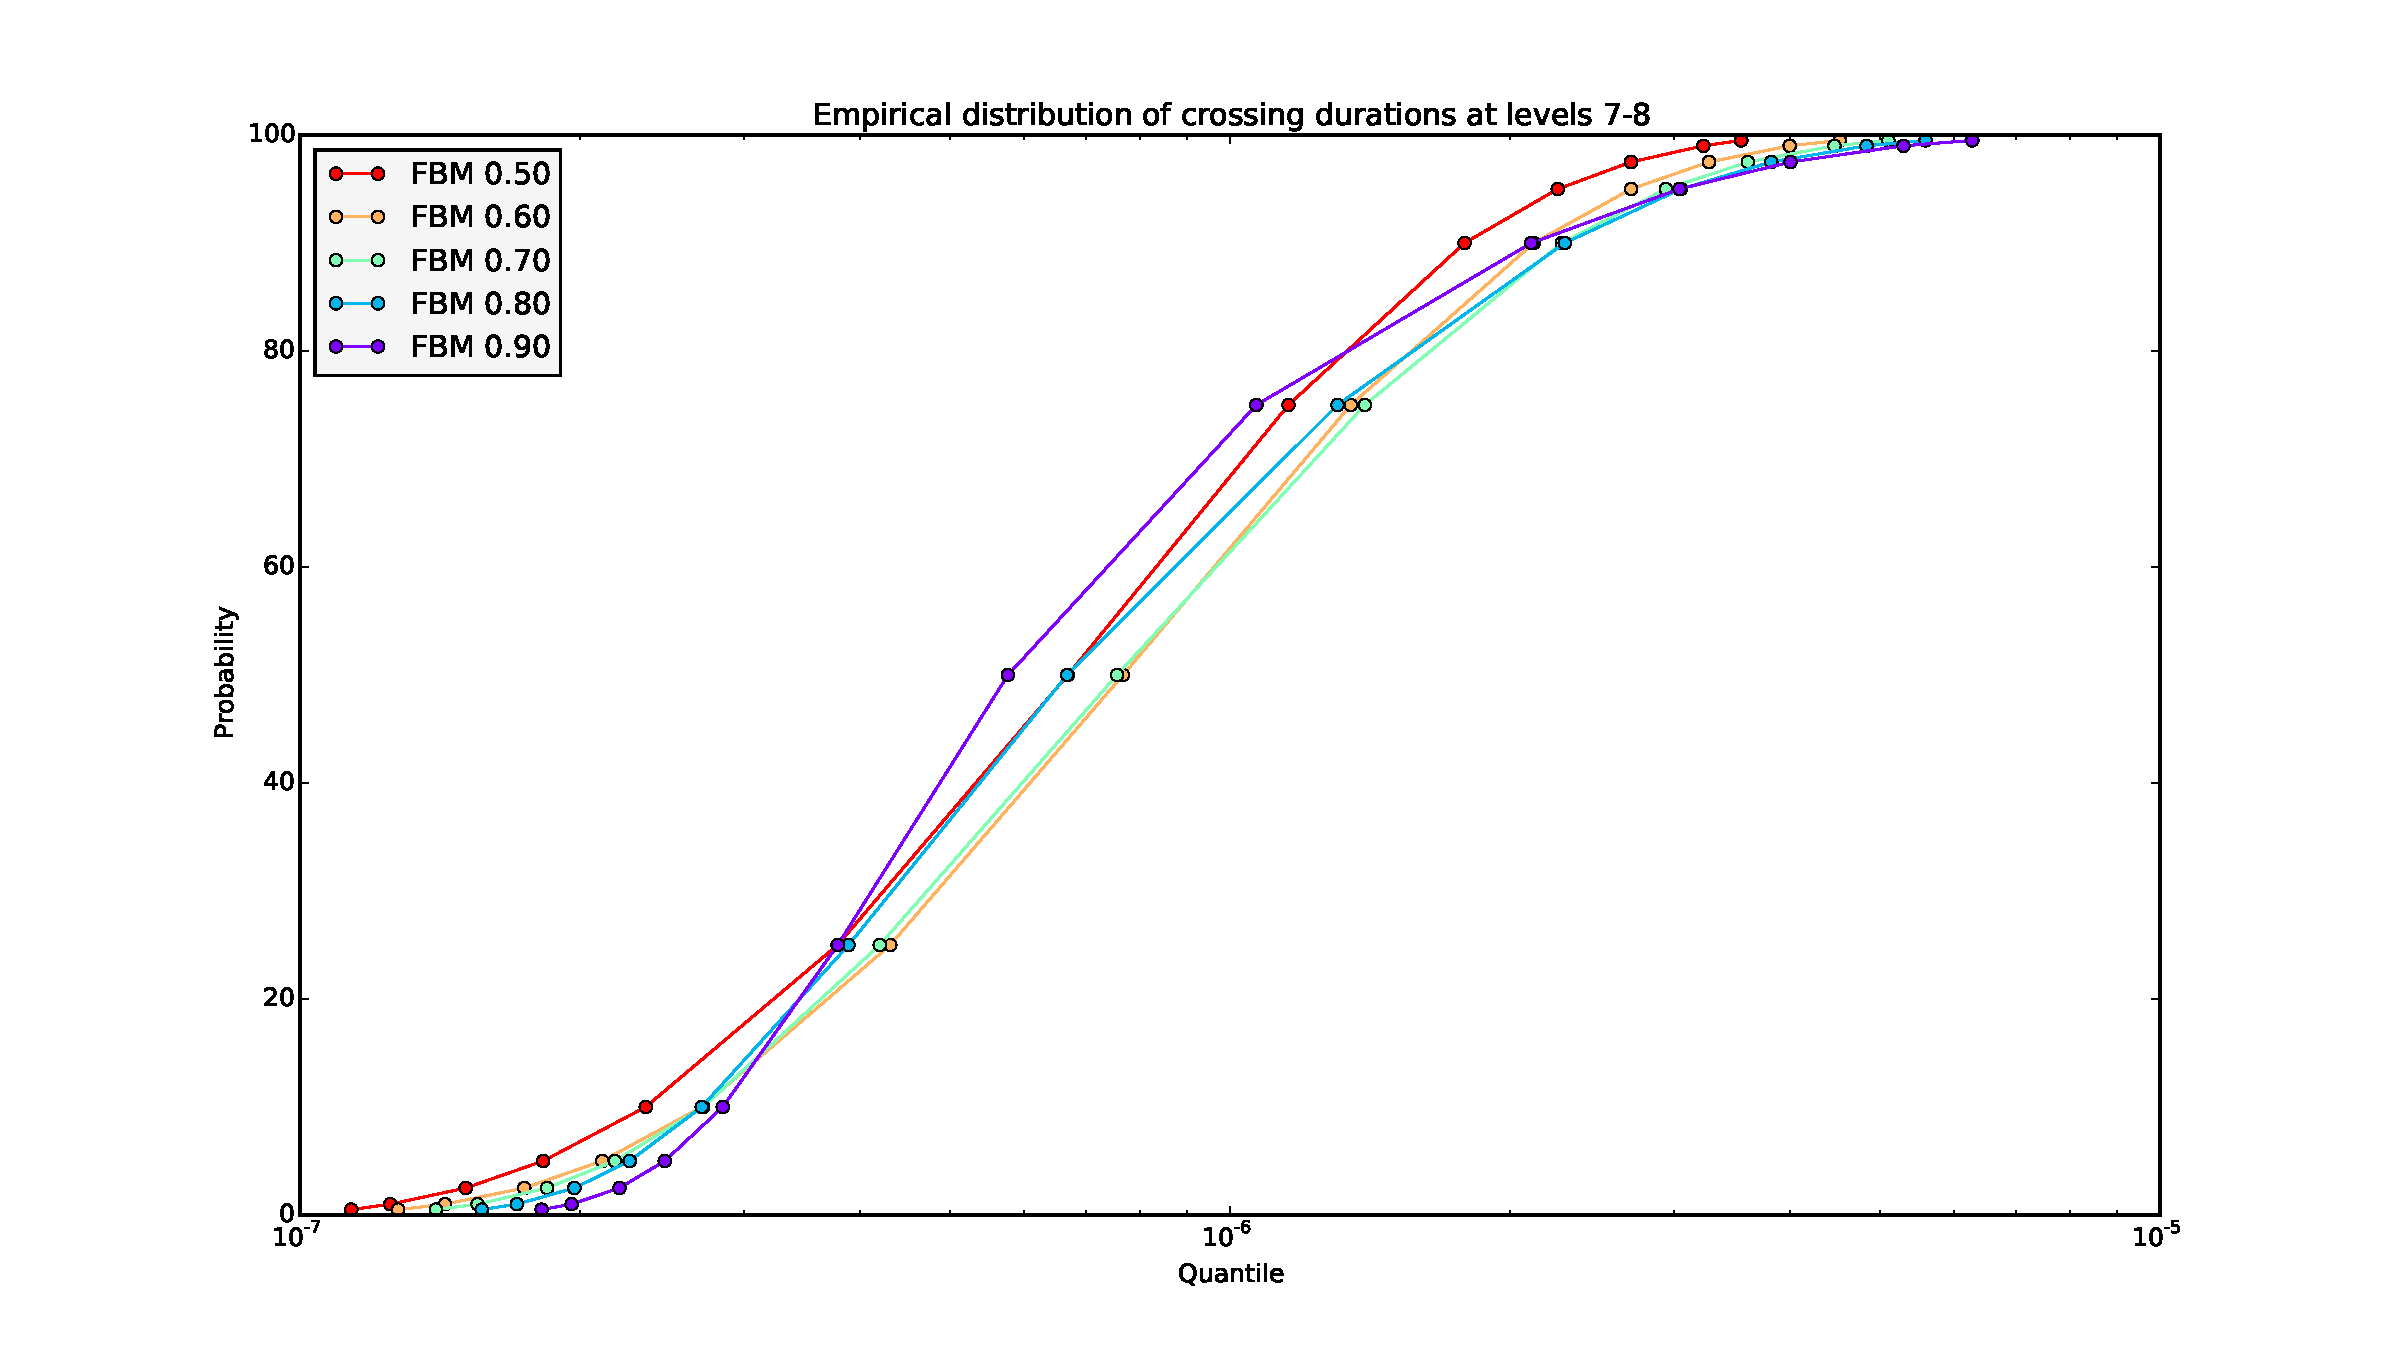
\includegraphics[width=6in]{images/fig_10_med_FBM}
    \caption{Empirical distributions of crossing durations estimated on levels 7-8
    for the fBm ($2^{21}$ datapoints). Averaged across all Monte-Carlo realisations.}
\label{fig:fbm_quantiles_durations}
\end{center}\end{figure}


% section results (end)

